\documentclass[a4paper,12pt, twoside]{article}
%layout packages
\usepackage{geometry} %Page layout
\geometry{a4paper, top=25mm, left=25mm, right=25mm, bottom=25mm,
         headsep=10mm, footskip=12mm}
\usepackage{lscape}
\usepackage{setspace} %linespacings
\onehalfspacing
\usepackage{graphicx}
\usepackage{color}
\usepackage{textcomp} %Celsius symbol, euro sign
\usepackage{amsmath} %formula
\usepackage{mathtools} %formula
\usepackage{url}
\usepackage{xfrac}
%\usepackage{showkeys} %zeigt keys der Bilder an, vor Endversion auskommentieren
\usepackage{listings} % f\"{u}r source code formatting
	\lstset{language=R,
		basicstyle=\footnotesize
		}
%\usepackage[toc,page]{Appendix}
\usepackage{verbatim} % enables to 'comment' entire paragraphs

% enables to run makeindex used for package{nomencl} from within latex document
\def\execute{%
\begingroup
\catcode`\%=12
\catcode`\\=12
\executeaux}
\def\executeaux#1{\immediate\write18{#1}\endgroup}
\usepackage[intoc]{nomencl}
%\execute{makeindex Masterarbeit.nlo -s nomencl.ist -o Masterarbeit.nls}
\renewcommand{\nomname}{Abbreviations} 	% changes name nomenclature to abbreviations
\setlength{\nomitemsep}{-\parsep}
\setlength{\nomlabelwidth}{.20\hsize}
\makenomenclature

%Figure packages
\usepackage{wrapfig} %erm\"{o}glicht, text um bilder flie\\ßen zu lassen
%\usepackage{subfig}
\usepackage{rotating} %damit bildunterschrift auch gedreht werden kann
\usepackage{graphicx} 
\usepackage{caption} 
\usepackage{subcaption}

%tabular packages
\usepackage{multirow}
%\usepackage{longTable}
\usepackage{array}
\usepackage{booktabs} %nice looking Tables
\usepackage[labelformat=simple, labelsep=colon, justification=justified, labelfont=bf, textfont=normalfont, font=small]{caption}
\captionsetup[lstlisting]{font=singlespacing} 

%new Table column types
\newcolumntype{R}[1]{>{\raggedleft\arraybackslash}#1}		%rechtsb\"{u}ndig
\newcolumntype{L}[1]{>{\raggedright\arraybackslash}#1}		%linksb\"{u}ndig
\newcolumntype{C}[1]{>{\centering\arraybackslash}#1}		%zentriertO


% other new commands
\newcommand{\HRule}{\rule{\textwidth}{0.5mm}}
\newcommand{\up}[1]{\ensuremath{^{\textrm{\tiny#1}}}}	% hochstellen im flie\\ßtext
\newcommand{\down}[1]{\ensuremath{_{\textrm{\tiny#1}}}}	% tiefstellen im flie\\ßtext
\newcommand{\beginsupplement}{%
        \setcounter{table}{0}
        \renewcommand{\thetable}{S\arabic{table}}%
        \setcounter{figure}{0}
        \renewcommand{\thefigure}{S\arabic{figure}}%
     }

% bib packages
\ProvidesFile{merlin.mbs}[2011/03/28 4.32 (PWD, AO, DPC)]
\usepackage{natbib}
\bibpunct{[}{]}{,}{a}{}{,}

\begin{document}
% Introduction
%\chapter{Introduction}

The field of quantitative genetics has come far since Fisher's initial studies on growth traits in wheat in 1918 \citep{}. While back then the concept of inheritance existed, little was known about the molecule responsible.  The discovery of the DNA structure by Franklin, Watson and Crick and technical break-throughs in analysing its sequence some xx years later, have allowed to investigate genetic variance on a much more detailed scale, moving from whole chromosomes and linkage studies to the analysis of DNA variation on a single-base pair level. The developments gentoyping and sequencing technologies in the recent years, have made large scale studies on genetic variation feasible. With the sinking costs of genotyping techniques, the number of samples investigated has risen and studies investigating effect of single DNA bases often comprise thousands of individuals, especially in the field of human genetics.  Together with the increased number of samples available in these studies, the number of phenotypes that are measured for each individual has grown from a few measurements to tens or even hundreds. The availability of these rich datasets provides great opportunities in studying genetic variations and its outcomes, such as studying pleiotropy and xx.  However, it also poses technical challenges in analysing these dataset. 

 Many cohort studies now have rich, high dimensional datasets ranging from studies in model organism such as yeast and arabidopsis thaliana to human molecular, morphological or imaging derived traits \citep{Bloom2013,Atwell2010,Astle2009,Shaffer2016,Stein2010}. However, these cohorts have often been analysed trait by trait partly for simplicity and partly because of a paucity of models suitable for the anlaysis of the high dimensional phenotype data.

\section{Multi-trait mapping}
Many cohort studies today, ranging from studies in model organism such as yeast and arabidopsis thaliana to human, have rich, high dimensional datasets including molecular, morphological or imaging derived traits \citep{Bloom2013,Atwell2010,Astle2009,Shaffer2016,Stein2010}. However, these traits have often been analysed separately,  partly for simplicity and partly because of a paucity of models suitable for the anlaysis of high-dimensional phenotype data. A variety of multi-trait models have been developed which can be broadly grouped into three different classes: i) dimensionality reduction techniques, ii) meta-analysis approaches and iii) multivariate regression models (reviewed in \citep{Shriner2012,Yang2012}). 
\paragraph{Dimensionality reduction techniques}  
Dimensionality reduction methods in genotype-phenotype mapping seek to find a linear combination of the phenotypes \(\mat{Y} \in \mathcal{R}^{N,P}\) into a lower dimensional space \(\tilde{\mat{Y}} \in \mathcal{R}^{N,K}\):
\begin{equation}
\tilde{\mat{Y}} = b_1\mat{y}_1 + b_2\mat{y}_2 + \dots + b_P\mat{y}_P
\end{equation}

Two commonly employed dimensionality reduction methods are principal component analysis (PCA) and canonical correlation analyses (CCA). In PCA, the components of the new phenotype representation are called principal components (PC) and are the eigenvectors \tmat{W} of the empirical covariance matrix \(\mat{Y}^T\mat{Y}\): \(\mat{Y}^T\mat{Y} = \mat{W}\mat{\Lambda}\mat{W}^T\). The eigenvalues \(\Lambda\) corresponding to the PCs are equivalent to the variance explained by their components. The transformation of the phenotype data into principal components leads to a projection where the highest amount of phenotypic variance explained lies in the first component, the second highest variance in the second component and so forth. The dimensionality reduction is achieved by using the first \(K\) principal components until the cumulative sum of the eigenvalues reaches a predefined threshold of total phenotypic variance that should be retained. These \(K\) principal components are used as proxy phenotypes for the association study. PCA as a dimensionality reduction technique has for instance been used in studies to find links between genotypes and facial features or obesity phenotypes \citep{Liu2012,Claes2014,He2008}. Recently, Aschard and colleagues \ref{Aschard2014} demonstrated that simply focusing on the principal components with the highest variance might not exploit the full potential of using PCA for genetic association. They propose a model of combined PCA where the PCs are grouped based on the level of variance they explain. They show a power gain in detecting genetic associations compared to simple approaches of only testing the top few PCs.

While the PCA dimensionality reduction approach focus on the phenotype space and subsequent association with the genotypes, CCA finds the optimal transformation of \tmat{Y} into \(\tilde{\mat{Y}}\) while simultaneously testing for the association with the genotypes. Originally proposed by Hotelling for any set of variables that remain invariant under internal linear transformation\citeyear{Hotelling1936}, in quantitative genetics CCA seeks to maximise the canonical correlation \(\hat{\rho}\) between  \(\tilde{\mat{Y}}= A^T\mat{Y}\) and a genotype \(\mat{X} \in \mathcal{R}^{N,1}\):   \(\hat{\rho} = cor(\mat{X},\tilde{\mat{Y}}) = \Sigma_{XY}A(A^T\Sigma_{YY}A\Sigma_{XX})^{-\frac{1}{2}}\). \(\Sigma_{YY},\Sigma_{XX} \text{ and } \Sigma_{XY}\) are the empirical sample covariance matrices of the phenotypes, the genotypes and cross-covariance of the phenotypes and genotypes, respectively. \(\hat{\rho}\) is maximised by finding the squared root of the largest eigenvalue of the \(\Sigma_{YY}^{-1}\Sigma_{YX}\Sigma_{XX}^{-1}\Sigma_{XY}\) covariance matrix and the corresponding eigenvector \tmat{A} contains the coefficients for constructing \(\tilde{\mat{Y}}\) \citep{Yang2102}. CCA finds the transformation \(\tilde{\mat{Y}}\) that explains the maximum amount of the covariation between the genotype and all traits. The significance of the correlation i.e. the genotype-phenotype association can be tested via Bartlett's likelihood ratio test with the null hypothesis of \(\text{H}_\text{0: }\Sigma_{YX} = 0\) \citep{Bartlett1941}. Ferreira and Purcell showed in simulations that CCA with multiple traits and one genetic marker \tmat{X} controls well for type I errors and has increased power compared to multivariate tests. In order to extend the CCA method to more than one marker, the genotypes also undergo a linear transformation: 
 \(\hat{\rho} = cor(B^T\mat{X},A^T\mat{Y}) = B^T\Sigma_{XY}A(A^T\Sigma_{YY}AB^T\Sigma_{XX}B)^{-\frac{1}{2}}\) and the maximum \(\hat{\rho}\) is found by solving for the largest eigenvalue of both \tmat{A} and \tmat{B}. As the number of genotype markers in GWAS exceeds the number of samples, estimates of the covariance matrix \(X^TX\) become unreliable \citep{Schaefer2005}. Several methods have been developed to circumvent this issue, making use of sparse matrices \citep{Parkhomenko2009} or a priori grouping of the genotypes \citep{Naylor2010}. 

 \paragraph{Meta-analysis approaches}
Meta-analysis approaches combine the simplicity of the univariate approaches with the advantages of the multivariate approach. For each phenotype, a univariate association study is conducted and the summary stastics of these tests combined. Many methods for combining the summary statistics \citep{Xu2003,Yang2010,Yang2012,Bolormaa2014} go back to the work by O'Brien \citep{O'Brien1984}, who proposed to use a linear combination of the observed test statistics for each univariate test \(\mat{T} =(T_1, \dots, T_P)^T\) as the new statistics to be evaluated for significance.  \tmat{T} is asymptoctically normal distributed with mean \(\mat{\mu} = (\mu_1,\ldots, \mu_P)^T\) and covariance matrix \(\mat{\Sigma}\). O'Brien stastistic allows for testing the Null hypothesis \(H_0: \mu = 0\) against the alternative hypothesis of  \(H_1: \mu_p \ge 0, p=1, \ldots , P \) and is most powerful if \(\mu_1= \ldots =\mu_P\) \citep{Xu2003}. It is defined as: \(S = \mat{J}^T \mat{\Sigma}\mat{T}\), with \(\mat{J} = (1, 1, \ldots, 1)^T\).  The statistic has been modified in a number of studies, by adapting either the weighting matrix \tmat{J}, the covariance matrix \tmat{\Sigma} or both. Xu and colleagues \citeyear{Xu2003} optimised \(S\) to allow for testing against a general \(\mu\) rather then for a case where  \(\mu_1= \ldots =\mu_P\) by allowing for flexible, but restrained weights in \tmat{J}. Similarily, Yang and colleagues  \citeyear{Yang2010} proposed non-uniform weights to reflect heterogeneity in the means and use a sample splitting and cross-validation approach to determine the optimal weights. 
While the previous two studies showed an increase in power for using the combined statistic, they either used a small marker set or small number of phenotypic traits.  Bolormaa and colleagues showed that these power gains also hold for genotype to phenotype mapping of 32 traits across all genome-wide markers \citep{Bolormaa2014}. In their study, the weights of O'Briens proposal are substituted by the signed t-statistic. 

\paragraph{Regression models} There are a number of different regression models that allow for the multivariate analysis of phenotypes. Among them are graphical models, generalized estimation equations and frailty models, for which a summary of methods and application can be found in \citep{Shriner2012,Yang2012}. Here, I will focus on describing the development of multivariate linear regression models for genotype-phenotype mapping. The underlying models and their derivation have been described in \cref{sec:intro}. Before the era of GWAS, QTL mapping in linkage experiments have demonstrated the increase in power when jointly analysing traits with common underlying genetics. Jiang and colleagues \citeyearpar{Jiang1995} proposed a multi-trait model where the phenotypes are jointly modeled as the sum of the fixed genetic effects of interest, fixed effects for genetic background variation and residual noise. They show that the joint analysis of traits can increase power to detect the underlying genetics and can increase the precision of the parameter estimates. The significance of the association is determined via a likelihood ratio test of the parameter estimates under the Null model where the fixed genetic effect is zero and the parameter estimates under the alternative model. The alternative model design depends on the underlying biological hypothesis regarding the effect of the genetic variant. Here, Jiang and colleagues differentiate hyptheses for a simple joint mapping of phenotypes, pleiotrophy and gene-environment interactions. Joint mapping does not make any assumptions about the underlying genetic architecture and simply tests if an association can be found when both traits are analysed jointly, i.e. the effect of the genetic variant is non-zero for at least one of the traits. This hypothesis can be extended in requiring that the effect on both traits is unequal to zero. In this case, the genetic variant is considered to be pleiotrophic. To test for gene-environment interaction, the different conditions a trait was studied in can be treated as different traits and be jointly mapped. If the effect size estimates of the genetic variant are not equal, the variant is considered to have environmental interactions.  Methods developed thereafter often use the same underlying hypotheses for the mapping, but different techniques for the evaluation of the significance. For instance, two other groups developed methods for the joint analysis of traits based specifically on the residual sum of squares (RSS) matrix of the standard linear model (\cref{eq:lm}) estimated at each locus tested \citep{Knott2000,Korol2001}. In the model proposed by Knott and Haley, the different properties and descriptors of the RSS are used to determine the significance of the QTL mapping. To test for pleiotropy for instance, the determinent of the RSS at the test locus is compared to the RSS of the null model of no association. In contrast, Korol and colleagues propose to use the RSS of the multi-trait mapping as a means for trait transformation and dimensionality reduction. The resulting one-dimensional trait per sample is fitted in a single-trait test for significance testing.  While methods described so far have only used fixed genetic effects, Korte and colleagues \citeyear{Korte2012} were the first to introduce a random genetic effect into the model. Based on the original model by Jiang, they substituted the fixed effect accounting for background genetics by a random effect, turning the multivariate linear model into a mulitvariate linear mixed model (Equation~\ref{eq:lmm}). Based on these principals and method development for the efficient analysis of large cohort sizes, a number of publically available frameworks for the genome-wide mapping of a moderate number of traits via multivariate linear mixed models were developed. \citep{Korte2012,Yang2011,Lippert2014,Zhou2014,Casale2015}. 

Out of the differerent approaches described above, multivariate linear mixed models (LMMs) have the additional advantage that they can control for population structure (\cref{sec:intro}). In LMMs, both the residual noise and the genetic backgound are modeled as random effects. For the random genetic effect, a complex covariance structure can be modeled such that family structure and relatedness captured in the genotypes can be exploited to model background genetic correlations in phenotype\citep{Yu2006,Kang2008} (\cref{eq:lmm}). The random effects are assumed to be composed of a sample-to-sample and trait-to-trait covariance component. The genetic sample covariance can be obtained from the data itself, e.g. using a genetic relationship matrix (GRM) or identity by descent, whereas the trait covariance terms need to be estimated from the observed data. Since the introduction of LMM for multi-trait GWAS studies, LMMs have been extended to handle the large sample sizes obtained in particular in human studies, allowing for cohort sizes of \red{xxx}  individuals \citep{Zhou2014}. However nearly all current methods scale poorly in the number of traits ($P$) due to a bottle neck caused by estimating the trait covariance terms. 

Together with Francesco Paolo Casale, a PhD student in Oliver Stegle's research group at the EBI, I developed a simple, but surprisingly effective heuristic which uses a linear mixed model with bootstrapping (LiMMBo) that allows for the analysis of datasets with a large number of phenotypic traits. In order to validate LiMMBo and show its applicability to high-dimensional phenotypes, I developed a phenotype simulation framework which allows for the simulation of well-defined phenotypes with different underlying genetic structures and noise distributions. This chapter describes this simulation strategy and the LiMMBo approach and its validity. 

\section{Genetic variation}
\section{Genome-wide association studies}
\begin{figure}[hbtp]
	\centering
	\includegraphics[trim = 0mm 0mm 0mm 0mm, clip, width=\textwidth]{Introduction/Figures/GenotypePhenotype.pdf}
	\caption[\textbf{.}]{\textbf{.} } 
	 	\label{fig:GenoPheno}
\end{figure}

\subsection{From genotype arrays to genome-wide SNP data}
\begin{itemize}
	\item Reference panel: HapMap, 1000Genomes, Uk10K
	\item Phasing and Imputation
\end{itemize}

\subsection{From molecular to organismal phenotypes}
\begin{itemize}
	\item eQTLs, eWAS
	\item intermediate phenotypes: organ level, brain, facial morpholgy
	\item case-control studies
\end{itemize}

\subsection{Linear Mixed Models}

Fixed genetic background componts are standardly modeled via principal components (PCs) of genotype data \citep{Price2006} and have been shown to adjust well for population structure based on ancestry differences \citep{Patterson2006}. However, PCs perform poorly in modeling family structure or cryptic relatedness.  By modeling genetic background as a random effect, more complex covariance structures can be used such that correlations in phenotype reflect family structure and relatedness \citep{Yu2006,Kang2008}.
	
Pruning for LD structure to construct kinship matrices \citep{Eu-ahsunthornwattana2014}
Derivation of kinship matrix as  \(\frac{1}{7}\) \citep{Speed2012}
	
\subsection{Linear models}
In genotype to phenotype mapping, the most simple linear model (LM) describes the linear relationship between a phenotype \(y\) and a genetic marker \(x\). Optionally, known covariates \(F\) can be included as explanatory variables. There are a variety of different types of models, depending on the structure of background effects and the number of phenotypes that are modeled simultaneously. In the following, a short description of the models relevant for this project is outlined. 

\label{sec:ssection:lm}
\paragraph{Uni-variate linear models for genetic analyses}
The uni-variate LM models a single phenotype \(y\) as the sum of a fixed effect of the genetic marker \(x\) and \(K\) known covariates \(F\) and residual noise \(\psi\) across \(N\) samples:

\begin{equation}
\mat{y} = \mat{F}\mat{\alpha} + \mat{x}mat{\beta} + \mat{\psi},\text{ }
\mat{\psi} \sim \normal 0 {\sigma_e^2\matsub{I}{N}}.
\label{eq:lm-uv}
\end{equation}

with
\begin{align*} 
& \text{the phenotype vector } \mat{y} \inR N 1,\\
& \text{the matrix of $K$ covariates }\mat{F} \inR N K,\\
& \text{the effect of covariates } \mat{\alpha} \inR K 1,\\
& \text{the genetic profile of the SNP being tested }\mat{x} \inR N 1 \text{and}\\
& \text{the effect size of the SNP } \mat{\beta} \inR x x \\
\end{align*} 


\noindent The association between phenotypes and the genetic markers can be assesed by testing the hypothesis that the genetic variant has an effect \(\beta \neq 0\) versus having no effect on the phenotype. The log likelihood ratio (LLR) test statistic \(\Lambda\) is a commonly used statistic to compare the likelihood of the full model \taltH (Equation~\ref{eq:lm-uv}) with \(\beta \neq 0\) to the one of the Null model \tnullH:
\begin{equation}
\nullH: \mat{y} =\mat{F}\mat{\alpha}  + \mat{\psi},\text{ }
\mat{\psi}\sim \normal 0 {\sigma_e^2\matsub{I}{N}}
\label{eq:lm_null}
\end{equation}

\noindent The LLR test statistic \(\Lambda\) is defined as
\begin{equation}
\Lambda  =  \mathcal{L} (\hat{\beta}, \hat{\alpha}, \hat{\sigma_{e}}) -  \mathcal{L} (0, \hat{\alpha}, \hat{\sigma_{e}})
\label{eq:llr}
\end{equation}

\noindent where \(\mathcal{L} (\hat{\beta}, \hat{\alpha}, \hat{\sigma_{e}})\) are the maximum likelihood estimators (MLE) of  \taltH and \(\mathcal{L} (0, \hat{\alpha}, \hat{\sigma_{e}})\) the MLE of \tnullH. 

\noindent \(2\Lambda\) follows a \(\chi^2_{df}\) distribution with \(df\) degrees of freedom \citep{Wilks1938} 
\begin{equation}
2\Lambda \sim \chi^2_{df} 
\label{eq:lambda}
\end{equation}

\noindent and allows for the calculation of the P value as :
\begin{equation}
P(\Lambda) = 1 - F_{\chi^2}(2\Lambda, df)
\label{eq:pvalue}
\end{equation}

\paragraph{Multi-variate linear models for genetic analyses.} Extending the model to a multi-variate linear model, i.e. jointly modeling multiple phenotypes \(P\), requires the introduction of trait-design matrices for the fixed effects (\(\mat{A}\) and \(\mat{B}\) for the covariate and genetic effect respectively) and a trait-by-trait covariance matrix \tmatsub{C}{n} for the residual noise:
\begin{equation}
\mat{Y} =\mat{F}\mat{A}\matsub{W}{\alpha} +\mat{x}\mat{B}\matsub{W}{\beta} + \mat{\psi},\text{ }
\mat{\psi}\sim \multinormal N P 0 {\matsub{C}{n} \otimes\matsub{I}{N}}
\label{eq:lm-mv}
\end{equation}

with
\begin{align*} 
& \text{the Kronecker product } \otimes \\
& \text{the phenotype matrix }\mat{Y} \inR N P,\\
& \text{the matrix of $K$ covariates }\mat{F} \inR N K,\\
& \text{the effect of covariates } \mat{A} \inR K M,\\
& \text{the trait design matrix of the covariates }\matsub{W}{\alpha} \inR M P,\\
& \text{the genetype vector of the SNP being tested }\mat{x} \inR N 1\\
& \text{the effect size of the SNP } \mat{B} \inR 1 L \text{and}\\
& \text{the trait design matrix of the genotype }\matsub{W}{\beta} \inR L P,\\
\end{align*} 

The trait design matrices \(\mat{W}_{\alpha}\) and \(\mat{W}_{\beta}\) allow different scenarios of the cross-trait architecture of the independent effects on the phenotype.  For instance, in an 'common effect' setup where the genetic variant is assumed to have the same effect across all traits,  \tmat{B} is equal to \(1_{1xP}\) (\(L=1\)). Allowing different effects across all traits corresponds to  \( \mat{B} =  \matsub{I}{P} \) (\(L=P\)). In such a `any effect' setup, the multi-trait modelling simply serves to increase power for detecting genetic variants. 

\subsection{Linear mixed models}
Linear mixed models (LMMs) include both fixed and random effects in the model. In genetics, LMMs can model both fixed genetics effects, i.e. single variants, and background genetic effects, i.e. controling for population structure and accounting for polygenic background \citep{Yu2006}. Population structure and relatedness between individuals can be captured in a genetic relatedness matrix, which accounts for the pairwise genetic similarity between individuals. The relatedness matrix is estimated as
 \begin{equation}
 R = \frac{1}{S}XX^T
 \label{eq:relatedness}
 \end{equation}
 where \(S\) is the number of SNPs used for the estimation and \(X\) is the \(S \times N\) genotype matrix. As described for the linear model, there are uni-variate and multi-variate LMM set-ups for genetic association analyses. 


\paragraph{Uni-variate LMM for genetic analyses.} The genetic background and residual noise are modeled as random effects with a scalar MLE for the genetic \(g\) and noise trait-variance \(\psi\),   \(\sigma_g^2\) and \(\sigma_e^2\):

\begin{equation}
\mat{y} =\mat{F}\mat{\alpha} +\mat{x}\beta +\mat{g}+\mat{\psi},\text{ }
\mat{g} \sim \normal 0 {\sigma_g^2\mat{R}},\text{ }
\mat{\psi} \sim\normal 0 {\sigma_e^2\mat{I}_N}
\label{eq:lmm-uv}
\end{equation}

with
\begin{align*} 
& \text{the phenotype vector }\mat{y} \inR N 1,\\
& \text{the matrix of $K$ covariates }\mat{F} \inR N K,\\
& \text{the effect of covariates } \mat{\alpha} \inR K 1,\\
& \text{the genetic profile of the SNP being tested }\mat{x} \inR N 1,\\
& \text{the effect size of the SNP } \mat{\beta} \inR x x \text{ and}\\
& \text{the sample relatedeness matrix }\mat{R} \inR N N,
\end{align*} 

\paragraph{Multi-variate LMM for genetic analyses.} In the multi-variate case, the MLE of the trait covariances are \(P\times P\) trait-by-trait covariance matrices \tmatsub{C}{g} and \tmatsub{C}{n} for the genetic and noise components, respectively (Equation \ref{eq:lmm-mv}).

\begin{equation}
\mat{Y} =\mat{F}\mat{A}\mat{W}_{\alpha} +\mat{x}\mat{B}\mat{W}_{\beta} +\mat{g}+\mat{\psi},\text{ }
\mat{g}\sim \multinormal N P 0 {\matsub{C}{g} \otimes \matsub{R}{N}},\text{ }
\mat{\psi}\sim \multinormal N P 0 {\matsub{C}{n} \otimes \matsub{I}{N}}
\label{eq:lmm-mv}
\end{equation}

with
\begin{align*} 
& \text{the Kronecker product } \otimes \\
& \text{the phenotype matrix }\mat{Y} \inR N P ,\\
& \text{the matrix of $K$ covariates }\mat{F} \inR N K,\\
& \text{the effect of covariates } \mat{A} \inR K M,\\
& \text{the trait design matrix of the covariates }\matsub{W}{\alpha} \inR M P,\\
& \text{the genetype vector of the SNP being tested }\mat{x} \inR N 1\\
& \text{the effect size of the SNP } \mat{B} \inR 1 L \text{and}\\
& \text{the trait design matrix of the genotype }\matsub{W}{\beta} \inR L P,\\
\end{align*} 

\begin{figure}[hbtp]
	\centering
	\includegraphics[trim = 0mm 0mm 0mm 0mm, clip, width=\textwidth]{Introduction/Figures/GWASstats.pdf}
	\caption[\textbf{.}]{\textbf{.} } 
	 	\label{fig:GWAs-stats}
\end{figure}



Under Hardy-Weinberg:
allele frequencies: 
\begin{equation}
p + q =1
\end{equation} 

genotype frequencies: 
\begin{equation}
p^2 + 2pq + q^2 = 1
\end{equation} 

additive genotype encoding, allele dosages: 
\(d(a_{alt},a_{alt}) = 0\) 
\(d(a_{alt},a_{ref}) = 1\) 
\(d(a_{ref},a_{ref}) = 2\) 

Expected genotype per SNP: 
\begin{equation}
E(x) =  d(a_{alt},a_{alt}) \times p^2 + d(a_{alt},a_{ref}) \times 2pq + d(a_{ref},a_{ref}) \times  q^2)
E(x) = 2pq + 2q^2 = 2(1-q)q + 2q^2 = 2q 
\end{equation}

Variance and standard deviation of genoytpe per SNP: 
\begin{equation}
Var(x) = E(x^2) - E(x)^2 = d(a_{alt},a_{alt})^2 \times  p^2 + d(a_{alt},a_{ref})^2  \times 2pq + d(a_{ref},a_{ref})^2  \times q^2 - (2q)^2 =  2q(1-q)
\end{equation}

\begin{equation}
\sigma(x) = \sqrt(Var(x)) = \sqrt(2q(1-q))
\end{equation}

standardised genotypes:
\(x_{SNP} = \frac{x_{SNP}-2q_{SNP}}{\sqrt{2q_{SNP}(1-q_{SNP})}}\)

normal distribution for phenotypes\\
In both data sets, we quantile-transformed each single pheno-
type to a standard normal distribution to guard against model misspecification. Although this strategy does not guarantee that the transformed phenotypes follow a multivariate normal distri- bution jointly, it often works well in practice when the number of phenotypes is small \citep{Stephens2013,Zhou2014}

Quantitative measurements of organisms have been a bedrock of genetics since the birth of this science \citep{FisherWheat}. One can measure many different traits of an organism and it is natural to want to jointly analyse the measurements to discover genetic loci, generically called multi-trait analysis. Many cohort studies now have rich, high dimensional datasets ranging from studies in model organism such as yeast and arabidopsis thaliana to human molecular, morphological or imaging derived traits \citep{Bloom2013,Atwell2010,Astle2009,Shaffer2016,Stein2010}. However, these cohorts have often been analysed trait by trait partly for simplicity and partly because of a paucity of models suitable for the anlaysis of the high dimensional phenotype data. For few traits, a variety of multi-trait models have been developed in quantitative genetics going back to the work of Jiang and collegues \citeyearpar{Jiang1995} first proposed a model for the joint analysis of quantitaive trait loci. Existing methods can be broadly grouped into three different classes of models: i) dimension reduction techniques (e.g. principal component analysis or canonical correlation analysis), ii) meta-analysis approaches and iii) multivariate models (reviewed in \citep{Shriner2012}). Linear mixed models (LMM) belong to the latter class and methods based thereon are appealing because they control for population structure and other confounding factors using an additional random-effect term in the model. Multi-trait generalizations of LMMs are based on modelling phenotypic covariance using a sum of fixed effects, and random effects, where the random effect component has a sample and trait-trait component. 
The sample covariance can be obtained from the genetic variation data itself, e.g. using realized relation or IBD, IBS. The trait-trait covariance needs to be estimates from the observed data, which is a bottle neck of existing methods. params scales quadratic in P. Forthermore, the computational complexity in P is .. 



Multiple measurements are often modelled as a sum of the SNP of interest and then often two additional components, one for other genetic loci and one for other non-genetic variance. These components can be modelled as either fixed or random effects. 

 Korte and colleagues were the first to combine one of these methods with GWAS statistical tools to allow for multi-trait linear-mixed modeling of paired-phenotypes on a genome-wide level \citeyearpar{Korte2012}. These models have been extended to handle the large sample sizes present in particular in human studies \citep{Zhou2014,Casale2015}, however nearly all current methods scale poorly in the number of  traits ($P$), with complexity of commonly used methods rangig to up to \(O(P^6)\). In practice this limits these methods to traits of 10 or less. 

Here we develop a simple, but surprisingly effective heuristic which uses a linear mixed models with bootstrapping (LiMMBo) that allows for the analyse of datasets with a large number of phenotypic traits. We show in simulations that the critical step of estimating the variance decompostion of phenotypes in its genetic and noise component via LiMMBo yields consistent results to exisiting methods when applied to dataset with moderate number of traits. However LiMMBo can scale up to far greater high-dimensional phenotypes. We show that linear mixed models for high-dimensional phenotypes are feasable when using LiMMBo for variance decomposition. To show the effectiveness of LiMMBo on real datasets, we analysed a publically available yeast quantitative trait dataset \citep{Bloom2013} with 41 measurements. We see both an increase in power compared to uni-variate models and explore the benefits of jointly modelling large numbers of traits in genetic studies.

\subsection{Imaging genetics}


% Chapter 1
%\chapter{LiMMBo}
\label{chapter:limmbo}
Multi-trait models have been used in quantitative genetics since the mid-1990ies \citep{Jiang1995} and a variety of flavors are available such as methods based on dimension reduction techniques (e.g. principal component analysis or canonical correlation analysis) and multivariate models (reviewed in \citep{Shriner2012}). Korte and colleagues were the first to combine one of these methods with GWAS statistical tools to allow for multi-trait linear-mixed modeling of paired-phenotypes on a genome-wide level \citeyearpar{Korte2012}. Modeling traits jointly can improve the statistical power by accounting for correlated background variation as well as by combining weak genetic effects across traits. Accounting for correlated background allows the observed variance of the phenotype to be decomposed into different variance components such as genetic and environment components \citep{Korte2012}. Most multi-trait linear mixed model (mtLMM) frameworks are optimised for large numbers of samples (N) and SNPs but are limited to a moderate number of phenotypic traits (P, usually less than 10), as complexity can reach up to \(O(P^6)\) \citep{Zhou2014,Casale2015}.  In studies with more than ten phenotypic traits, alternative methods such a meta-analysis of single-trait setups have been applied \citep{Bolormaa2014}. I investigated different linear model set-ups for analysing datasets of more than 30 traits depending on the relatedness and population structure of the test cohort and complexity of the traits. Suitability of different methods was assessed by testing calibration of the models under the null hypothesis of no genetic association on simulated datasets with differing levels of relatedness and population structure. I developed a linear mixed model bootstrapping (LiMMBo)-based method that can analyse datasets with more than 30 phenotypes in a mtLMM framework when applicable. An increase in power compared to uni-variate models is demonstrated on a publically available yeast data set of 41 previously published quantitive traits \citep{Bloom2013}, by comparing the results of single-trait (st) to multi-trait (mt) GWAS. I show both in simulation and in real datasets that this estimation gives similar results for up to 30 phenotypes, but can scale up to 100 phenotypes.



%\section{Data simulation}
\label{section:simulation} 
Often, a first step in new method development is to reverse the task of genotype to phenotype mapping. The latter is commonly realised by fitting a linear model to the phenotype measurements and treating the genotype and possible covariates as explanatory variables. In order to evaluate new methods, one needs to have a set of well-characterised genotypes and phenotypes to know the ground truth based on which comparisons of the model performance can be made. Based on the underlying linear association methods, the phenotypes are often simulated as a linear composition of different effect components. 

For the methods development and selection process in this thesis (Section~\ref{section:limmbo} and \ref{sec:dimreduction}), I needed well-characterised phenotypes for evaluation before applying the methods to real datasets and biological questions. In the following section, I will first describe the simulation of genotypes with different levels of population structure and relatedness, followed by a description of the phenotype simulation. The simulation strategies described in this section apply to all simulated datasets within this thesis. 

\subsection{Genotypes}
\label{subsection:genotypes}
Genotypes can either be generated by sampling from real data sets or by simulating SNPs anew. In the latter case, assuming bi-allelic SNPs, each SNP is simulated from a binomial distribution with two trials and probability equal to the given allele frequencies  This simple approach, however, does not account for any LD structure in the genome. In contrast, sampling from a diverse set of real genotypes does not only facilitate retaining realistic LD structure in the genotypes, it also allows for the simple simulation of more defined population structure and relatedness within a cohort. As I wanted to evaluate the methods described in this thesis across different levels of relatedness and population structure, 
I chose to simulate the genotypes based on real genotype data from four European ancestry populations of the 1000 Genomes (1KG) Project (populations: CEU, FIN, GBR, TSI) \citep{Abecasis2012}, similar to strategies described in \citep{Loh2014,Casale2015}. I simulated three genotype sets, each with 1,000 samples, that differed i) in the number of ancestors \(N\) from which the genotypes were chosen and ii) the subpopulations the ancestors were chosen from:
\begin{enumerate}
\item unrelatedPopStructure: unrelated individuals with prior assigment of ancestral population  (\(N=10\))
\item unrelatedNoPopStructure: unrelated individuals with mixed ancestral population  (\(N=10\))
\item relatedNoPopStructure: related individuals with mixed ancestral population (\(N=2\))
\end{enumerate}

The number of ancestors sets the the level of relatedness within a cohort, where low numbers of \(N\) introduce relatedness among individuals, while high numbers of \(N\) lead to low levels of structure and relatedness. The choice of ancestrial population determines the level of subpopulation formation in the simulated genotypes: allowing for random selection of ancestors independent of the four subpopulations in the 1KG datasets yields low levels of population structure, whereas choosing ancestors based on their subpopulation gives rise to subpopulations in the simulated dataset as well. 
For the simulation, each newly synthesised individual is assigned to \(N\) ancestors from the original 1KG Project and their genome split into blocks of 1,000 SNPs. For each SNP block, an ancestor is chosen at random either from the whole dataset (NoPopstructure) or a subpopolution (Popstructure)  and its genotype is copied to the individuals genome. 

The level of structure and relatedness introduced by this simulation strategy can be visualised by examining the GRM and the principal components of the genotypes. The kinship as estimated via Equation~\ref{eq:kinship} is a measure of relatedness between the individuals, while principal components reflect the genotypic variance in the data. The hierarchical clustering of the genetic relationship estimates and scatter plots of the first two principal components for each genotype set are shown in Figure~\ref{fig:kinship-matrices}. Samples cluster tightly based on their ancestrial subpopulations (Figure~\ref{fig:kinship-matrices}A), while there is no clustering and an even spread in the PC plot for the cohort of unrelated individuals with ancestors sampled across all subpopulations (Figure~\ref{fig:kinship-matrices}B). The cohort of related individuals shows less spread in the second principal component and higher individual genetic relationship  estimates (Figure~\ref{fig:kinship-matrices}C).


\begin{figure}[!h]
	\centering
	\includegraphics[page=2, trim = 0mm 10mm 15mm 0mm, clip, scale=0.25]{Chapter1/Figures/simulatedCovarianceMatrices_kinship.png}
	\caption[Genetic relationship matrices and principal components of three simulated European ancestry cohorts]{\textbf{Genetic relationship matrices and principle components of three simulated European ancestry cohorts.} The genotypes were simulated based in genotype data from four European ancestry populations (ancestry colour key in panel A). Depending on the choice and number of ancestors for the sampling of chromosomes to simulate an individual's genotype, cohorts with differing levels of population and relatedness structure will arise. The left column depicts the hierarchical clustering of the sample-to-sample  genetic relationship coefficients (complete linkage clustering of euclidean distance between coefficients), the right column the first and second principal component (PC) of the sample genotypes for the three different cohorts: A. unrelated individuals, with population structure: \(N=10\), prior assigment to ancestral population; B. unrelated individuals, no population structure: \(N=10\), no prior assigment to ancestral population; C. related individuals, no population structure: \(N=2\), no prior assigment to ancestral population.}
 	\label{fig:kinship-matrices}
\end{figure}


\subsection{Phenotypes}
\label{subsection:phenotypes}
The simulation of phenotypes and their components can be described on two levels, either based on the biological meaning they reflect or the statistical type of the effect. In statistics, one distinguishes the fixed effects which are constant across individuals, from random effect which can vary (discussed in detail in \citep{Gelman2005}). On the biological level, we can classify the phenotypic components into genetic and non-genetic (noise) components.
Commonly simulated phenotype components are fixed and random genetic effects and fixed, correlated and random noise effects (e.g.\citep{Stephens2013,Marigorta2014,Zhou2014,Loh2014}). 

Genetic fixed effects are the effects of interest in genetic association studies i.e. the SNPs that are significantly associated with a phenotype. Genetic effects that are not associated on a per-SNP basis but reflect underlying population structure and relatedness in a cohort are simulated as random genetic effects. These effects are based on genetic relationship estimates or IBD which can be derived from the samples' genotypes. Non-genetic effects are used to simulate environmental, experimental or noise effects. Fixed noise effects are use to simulate confounding variables or covariates in an analysis, such as sex, age, weight or disease status. When simulating such confounding structures, assumptions about their distribution have to be made and this choice depends on the specific biological effects that should be modeled. Common distribution are binomial (e.g. sex), normal or uniform distribution (e.g. weight, height) or categorical (e.g disease status). Random noise effects simulate any non-specified noise effects that could arise due to, for instance, experimental measurement error.  Correlated noise effects are a type of random effect that can be used to simulate a phenotype component with a defined level of correlation between traits. For instance, such effects can reflect correlation structure decreasing in phenotypes with ordered or spatial components e.g. in imaging data. 

In addition to the different sources of variation these components model, they can further differ in their effect distribution across the simulated traits and the proportion of the variance they explain out of the total phenotypic variance. The simulation strategy of these components, the effect distribution and the scaling of the components to a specifc proportion of variance are described below. 
\\
\\
The phenotypes \( \mat{Y} \in \mathcal{R}^{N,P}\) of \(N\) samples and \(P\) traits are generated as the sum of i) fixed genetic effects \( \mat{U} \in \mathcal{R}^{N,P}\) , ii) random genetic effects \( \mat{G} \in \mathcal{R}^{N,P}\), iii) fixed noise effects \( \mat{C} \in \mathcal{R}^{N,P}\), iv) random noise effects \( \mat{\Psi} \in \mathcal{R}^{N,P}\) and v) correlated noise effects \( \mat{T} \in \mathcal{R}^{N,P}\). For component i-iv, a certain percentage of their variance is shared across all traits (shared) and the remainder is independent (ind) across traits.

\begin{enumerate}
\item \textit{Fixed genetic effects:} For the fixed genetic effects, \(S\) random SNPs for \(N\) samples are drawn from the simulated genotypes. From the \(S\) random SNPs, a proportion \tbm{\theta} is selected to be causal across all traits. \(\mat{U}^{\text{shared}} \in \mathcal{R}^{N,P}\) is simulated as the matrix product of this shared causal SNP matrix \(\mat{X}^{\text{shared}} \in \mathcal{R}^{N,\theta  \times S}\) and the shared effect size matrix \(\mat{B}^{\text{shared}} \in \mathcal{R}^{\theta  \times S, P}\) . \(\mat{B}^{\text{shared}}\) in turn is the matrix product of the two normally distributed vectors \(b_s \in \mathcal{R}^{\theta  \times S,1}\) and \(b_p^T \in \mathcal{R}^{1,P}\). The remaining \((1- \theta ) \times S\) SNPs are simulated to have an independent effect across a limited number of traits \(p^{\text{ind}}\). To realise this structure, \(\mat{B}^{\text{ind}}  \in \mathcal{R}^{(1-\theta)  \times S, P}\) is initialised with normally distributed entries. Subsequently, \(1 - p^{\text{ind}}\) traits are randomly selected and the row entries for \(\mat{B}^{\text{ind}}\) at these traits set to zero. \(\mat{U}^{\text{ind}} \in \mathcal{R}^{N,P}\) is the matrix product of  \(\mat{X}^{\text{ind}} \in \mathcal{R}^{N,(1 - \theta)  \times S}\)  and \(\mat{B}^{\text{ind}}\).
The fixed genetic effect \tmat{U} is the sum of \(\mat{U}^{\text{shared}}\) and \(\mat{U}^{\text{ind}}\).

\item \textit{Fixed noise effects:} The fixed noise effects \tmat{C} are based on \(K\)  confounders \(\mat{F} \in \mathcal{R}^{N,K}\), with a proportion \(\gamma\) being shared across all traits yielding the shared confounder matrix \(\mat{F}^{\text{shared}} \in \mathcal{R}^{\gamma \times K, P}\). The proportion of \(1- \gamma\) confounder that are independent make up the independent confounder matrix \(\mat{F}^{\text{ind}} \in \mathcal{R}^{(1-\gamma)  \times K, P}\). The distributions for each of the \(K\)  confounders are independent and can be either normal, uniform, binomial or categorical.  The effect size matrices  \(\mat{A}^{\text{shared}}  \in \mathcal{R}^{\gamma \times K, P}\)  and \(\mat{A}^{\text{ind}}  \in \mathcal{R}^{(1-\gamma) \times K, P}\) were designed as described for the fixed genetic effects. The total fixed noise effect is then \(\mat{C} = \mat{K}^{\text{shared}}\mat{A}^{\text{shared}} +  \mat{K}^{\text{ind}}\mat{A}^{\text{ind}}\).

\item \textit{Random genetic effects:} The random genetic effects \(\mat{G} \in \mathcal{R}^{N,P}\) are modeled as a matrix-normally distributed random variable, defined by its mean \(\mat{M} \in \mathcal{R}^{N,P}\), its column covariance \(\mat{C} \in \mathcal{C}^{P,P}\) and its row covariance \(\mat{D} \in \mathcal{R}^{N,N}\).  
\begin{equation}
\mat{G} \sim \matrixnormal N P M D C
\end{equation}
%\mat{M} \mat{R} mat{C}
The \(N \times N\) genetic relationship matrix \tmat{R}, estimated according to Equation~\ref{eq:kinship} from the SNP genotypes (of the simulated samples) represents the row covariance \tmat{D}.  The structure of the trait-to-trait covariance \tmat{C} depends on the design of the covariance effect, which can be either shared or independent across traits. To construct \tmat{G} from shared and independent random genetic effects, assume a matrix-normally distributed random variable \tmat{Z} with \(\mat{M}=0\)  and \(\mat{D} = \mat{R}\):

\begin{equation}
\mat{Z} \sim  \matrixnormal N P 0 R C
\end{equation}

\tmat{Z} can be expressed in terms of a multivariate normal distribution 

\begin{equation}
\text{vec}(\mat{Z}) \sim \multinormal N P {\mat{0}} {\mat{C} \otimes \mat{R}}.
\end{equation}

With the cholesky decompositon of \tmat{K} and \tmat{C} into  \(\mat{E}=\mat{BB}^T\) and \(\mat{C}=\mat{AA}^T\) 

\begin{equation}
\text{vec}(\mat{Z}) \sim \multinormal N P {\mat{0}} {\mat{AA}^T  \otimes \mat{BB}^T},  
\end{equation}

which can be rearranged  as with \tmat{I} as the identity matrix

\begin{equation}
\begin{aligned}
\text{vec}(\mat{Z}) \sim \multinormal N P {\mat{0}} {(\mat{A} \otimes \mat{B}) \mat{I} (\mat{A}^T \otimes \mat{B}^T)} \\
\text{vec}(\mat{Z})  \sim \multinormal N P {\mat{0}} {(\mat{A }\otimes \mat{B}) \mat{I} (\mat{A} \otimes\mat{B})^T)}.
\end{aligned}
\end{equation}

Using the property of a normally distributed random variable \tmat{Y} with mean \tmat{\mu} and covariance matrix \tmat{\Sigma}
\begin{equation}
\begin{aligned} 
w \mat{Y} \sim \normal {w\mat{\mu}}  {w\mat{\Sigma} w^T},
\end{aligned}
\end{equation}

we can let  \(\text{vec} (\mat{Z}) =  (\mat{A} \otimes \mat{B}) \text{vec} (\mat{Y})\)  and \(\mat{Y} \sim \multinormal N P {\mat{0}} {\mat{I}}\) such that
\begin{equation}
\begin{aligned}
(\mat{A} \otimes\mat{B}) \text{vec} (\mat{Y})  \sim \multinormal N P {\mat{0}} {(\mat{A} \otimes \mat{B}) \mat{I} (\mat{A} \otimes \mat{B})^T}
\end{aligned}
\end{equation}

Using \citep{Horn1991}: Lemma 4.3.1, we get 
\begin{equation}
(\mat{A} \otimes \mat{B}) \text{vec}(\mat{Y}) = \text{vec}(\mat{BYA}^T) 
\end{equation}

For the independent effect, \(\mat{A}^{\text{ind}}\) is a diagonal matrix with normally distributed entries: \((\mat{A}^{\text{ind}})^T = \text{diag}(a_1, a_2,  \dotsc , a_P) \sim \normal 0 1\), such that \(\mat{G}^{\text{ind}} =  \text{vec}(\mat{BY}(\mat{A}^{\text{ind}})^T) \). \(\mat{A}^{\text{shared}}\) of the shared effect is a matrix of row rank one, with normally distributed entries in row 1 and zeros elsewhere: \(a_{1,j} \sim \normal 0 1\) and \(a_{i \neq 1,j} = 0\) such that \(\mat{G}^{\text{shared}} =  \text{vec}(\mat{BY}(\mat{A}^{\text{shared}})^T) \). The total random genetic effect \tmat{G} is \(\mat{G} = \mat{G}^{\text{shared}} + \mat{G}^{\text{ind}}\). 

\item \textit{Random noise effects:} The random noise effects \tmat{\Psi} are simulated as the sum of a shared and an independent random noise effect. The shared random effect \(\mat{\Psi}^{\text{shared}}\) is simulated as \(\text{vec}(\mat{\Psi}^{\text{shared}}) \sim \normal 0 1\). The independent random effect \(\mat{\Psi}^{\text{ind}}\) is simulated as the matrix product of two normally distributed vectors \(\mat{a} \sim \multinormal N 1 0 1\) and \(\mat{b} \sim \multinormal P 1 0 1\): \(\mat{\Psi}^{\text{ind}} = \mat{ab}^T\).


\item \textit{Correlated noise effects:}  Correlated noise effects are simulated as a multivariate normal distribution with a covariance matrix described by the trait-trait correlation. The trait-trait correlation matrix \mat{C} is constructed as follows: traits of distance \(d=1\) (adjacent trait columns) will have the highest specified correlation \(r\), traits with \(d=2\) have a correlation of \(r^2\), up to traits with \(d=(P - 1)\) with a correlation of \(r^{(P - 1)})\) , such that the correlation is highest at the first off-diagonal element and decreases exponentially by distance from the diagonal. The final correlated noise effect matrix is simulated as \(\mat{T} \sim \multinormal N P {\mat{0}} {\mat{C}}\).
\end{enumerate}

Before combining the different components into the final phenotype, each component is rescaled by a factor \(a\) such that their average column variance explains \(x\) percent of the total variance. The scale factor \(a\) is derived as follows: 
Let \(X\) be a random variable with expected value \(E[X] = \mu_{x}\) and variance \(V[X] = E[(X - \mu_{x})^2]\) and let  \(Y = aX\). Then
  
\begin{equation}
\begin{aligned}
E[Y] &= a\mu_{x} \\
V[Y] &= E[(Y - \mu_{y})^2] \\
V[Y] &= E[(aX - a\mu_{x})^2] \\
		&= a^2 E[(X - \mu_{x})^2]. \\
\end{aligned}
\end{equation}

Hence, the scaling of a random variable by \(a\) leads to the scaling of its variance by \(a^2\). To scale the phenotype components such that their average column variance \(\overline{V_{col}} = \frac{V_1 + ... + V_p}{p} \) explains a specified  percentage \(x\) of the total variance, choose the scaling factor \(a\) such that: 
\begin{equation}
\begin{aligned}
x  &= a^2 \times \overline{V_{col}} \\
a  &= \sqrt{\frac{x}{\overline{V_{col}}}}
\end{aligned}
\end{equation}

The final simulated phenotype is expressed as
\begin{equation}
\mat{Y} = \mat{U}^{\text{scaled}}   + \mat{C}^{\text{scaled}} +  \mat{G}^{\text{scaled}} +  \mat{\Psi}^{\text{scaled}} + \mat{T}^{\text{scaled}}. 
\end{equation}

In Figure~\ref{fig:simulation}, I show an example of a simulated phenotype and its different components based on the simulation strategy described above. The phenotype consists of five traits for each of the 1,000 samples from a cohort of related individuals with no population structure. There are a total of ten causal SNPs and four covariates associated with the phenotype. In addition, it is composed of background genetic and noise effects as well as a correlated noise effect (correlation: 0.8). The total genetic variance accounts for 60\% of the variance leaving 40\% of variance explained by the noise terms.

\begin{figure}[hbtp]
	\centering
	\includegraphics[trim = 0mm 0mm 0mm 0mm, clip, width=\textwidth]{Chapter1/Figures/simulatedPhenotypes.png}
	\caption{\textbf{Phenotype simulation.} Heatmaps of the trait-to-trait correlation (Pearson correlation) of a simulated phenotype and its five phenotype components: fixed (fixedGenetic) and random (randomGenetic) genetic effects and fixed (fixedNoise), random (randomNoise) and correlated (correlatedNoise) noise effects. The fixed noise effects consist of four independent components, two following a binomial and two following a normal distribution, the fixed genetic effect of ten causal SNPs. The highest correlation for the correlated noise effect was set at 0.8. Apart from the correlated noise component, each component was simulated with 80\% of its variance shared across all traits, while the rest remained independent. The total genetic variance accounted to 60\% leaving 40\% of variance explained by the noise terms.}
	\label{fig:simulation}
\end{figure}


Developing new methods in quantitative genetics often requires simulated datasets with a well-characterised phenotype structure. Thereby, the number of phenotype components and their contribution to the final phenotypic variants depend on the task at hand. In order to provide a tool for phenotype simulation that is easily accessible and allows flexible simulation set-ups, I turned this simulation framework into the R package \textit{PhenotypeSimulator}, which can be installed from the Comprehensive R Archive Network  \citep{Meyer2017} \red{describe in more detail?}.


\section{Case study: multitrait GWAS of 41 growth traits in \emph{Saccharomyces cerevisiae}}
Things to elaborate on further:
\begin{itemize}
\item missing data and imputation: MAR, NMAR; One crucial parameter in the imputation strategy are the number of predictor variables one choses for the imputation of a given target variable. As a general rule, using every bit of available information yields multiple imputations that have minimal bias and maximal certainty (Meng 1995; Collins et al. 2001). This principle implies that the number of predictors should be chosen as large as possible. Including as many predictors as possible tends to make the MAR assumption more plausible, thus reducing the need to make special adjustments for NMAR mechanisms (Schafer 1997).
\item 'multivariate imputations by chained equations (MICE) \citep{vanBuuren2011}, which generates imputations for incomplete multivariate data by Gibbs sampling.
\item The imputation itself was done by predictive mean matching (PMM) \citep{Little1988}. PMM is a semi-parametric imputation method which can preserve non-linear relations in the data. 
\item multiple testing correction: Bonferroni, Benjamini and Hochberg, effective number of tests
\end{itemize}
The yeast dataset from a study by Bloom and colleagues \citeyearpar{Bloom2013} is used as case study dataset to show the feasibility of LiMMBo.

\subsection{Data}
\paragraph{Public dataset} The dataset consists of phenotype and genotype data of 1,008 prototrophic haploid \emph{Saccharomyces cerevisiae} segregants derived from a cross between a laboratory strain and a wine strain strains. It contains 11,623 unique genotypic markers obtained via short-read sequencing for all 1,008 segregants (no missing genotypes). For phenotyping, they grew segregants on agar plates under 46 different conditions, including different temperatures, pH and nutrient addition (see labels in Figure~\ref{fig:traitcorrelations}). The phenotypes were definded as end-point colony size normalized relative to growth on control medium. For the remainder of this chapter, a trait is defined as the normalised growth size in one conditions.
\paragraph{Phenotype imputation. } Out of the 1,008 segregants, 303 were phenotyped for all 46 traits. Missing phenotypes are not evenly distributed with some traits such as cobalt chloride being present for almost all samples and others such as sorbitol or raffinose are lacking in more than a third of the samples. The distribution of trait missingness across all samples is depicted in Figure~\ref{fig:missingness-all}. 

\begin{figure}[!h]
	\centering
	\begin{subfigure}[b]{0.48\textwidth}
		%\hspace{3cm}
		\center
	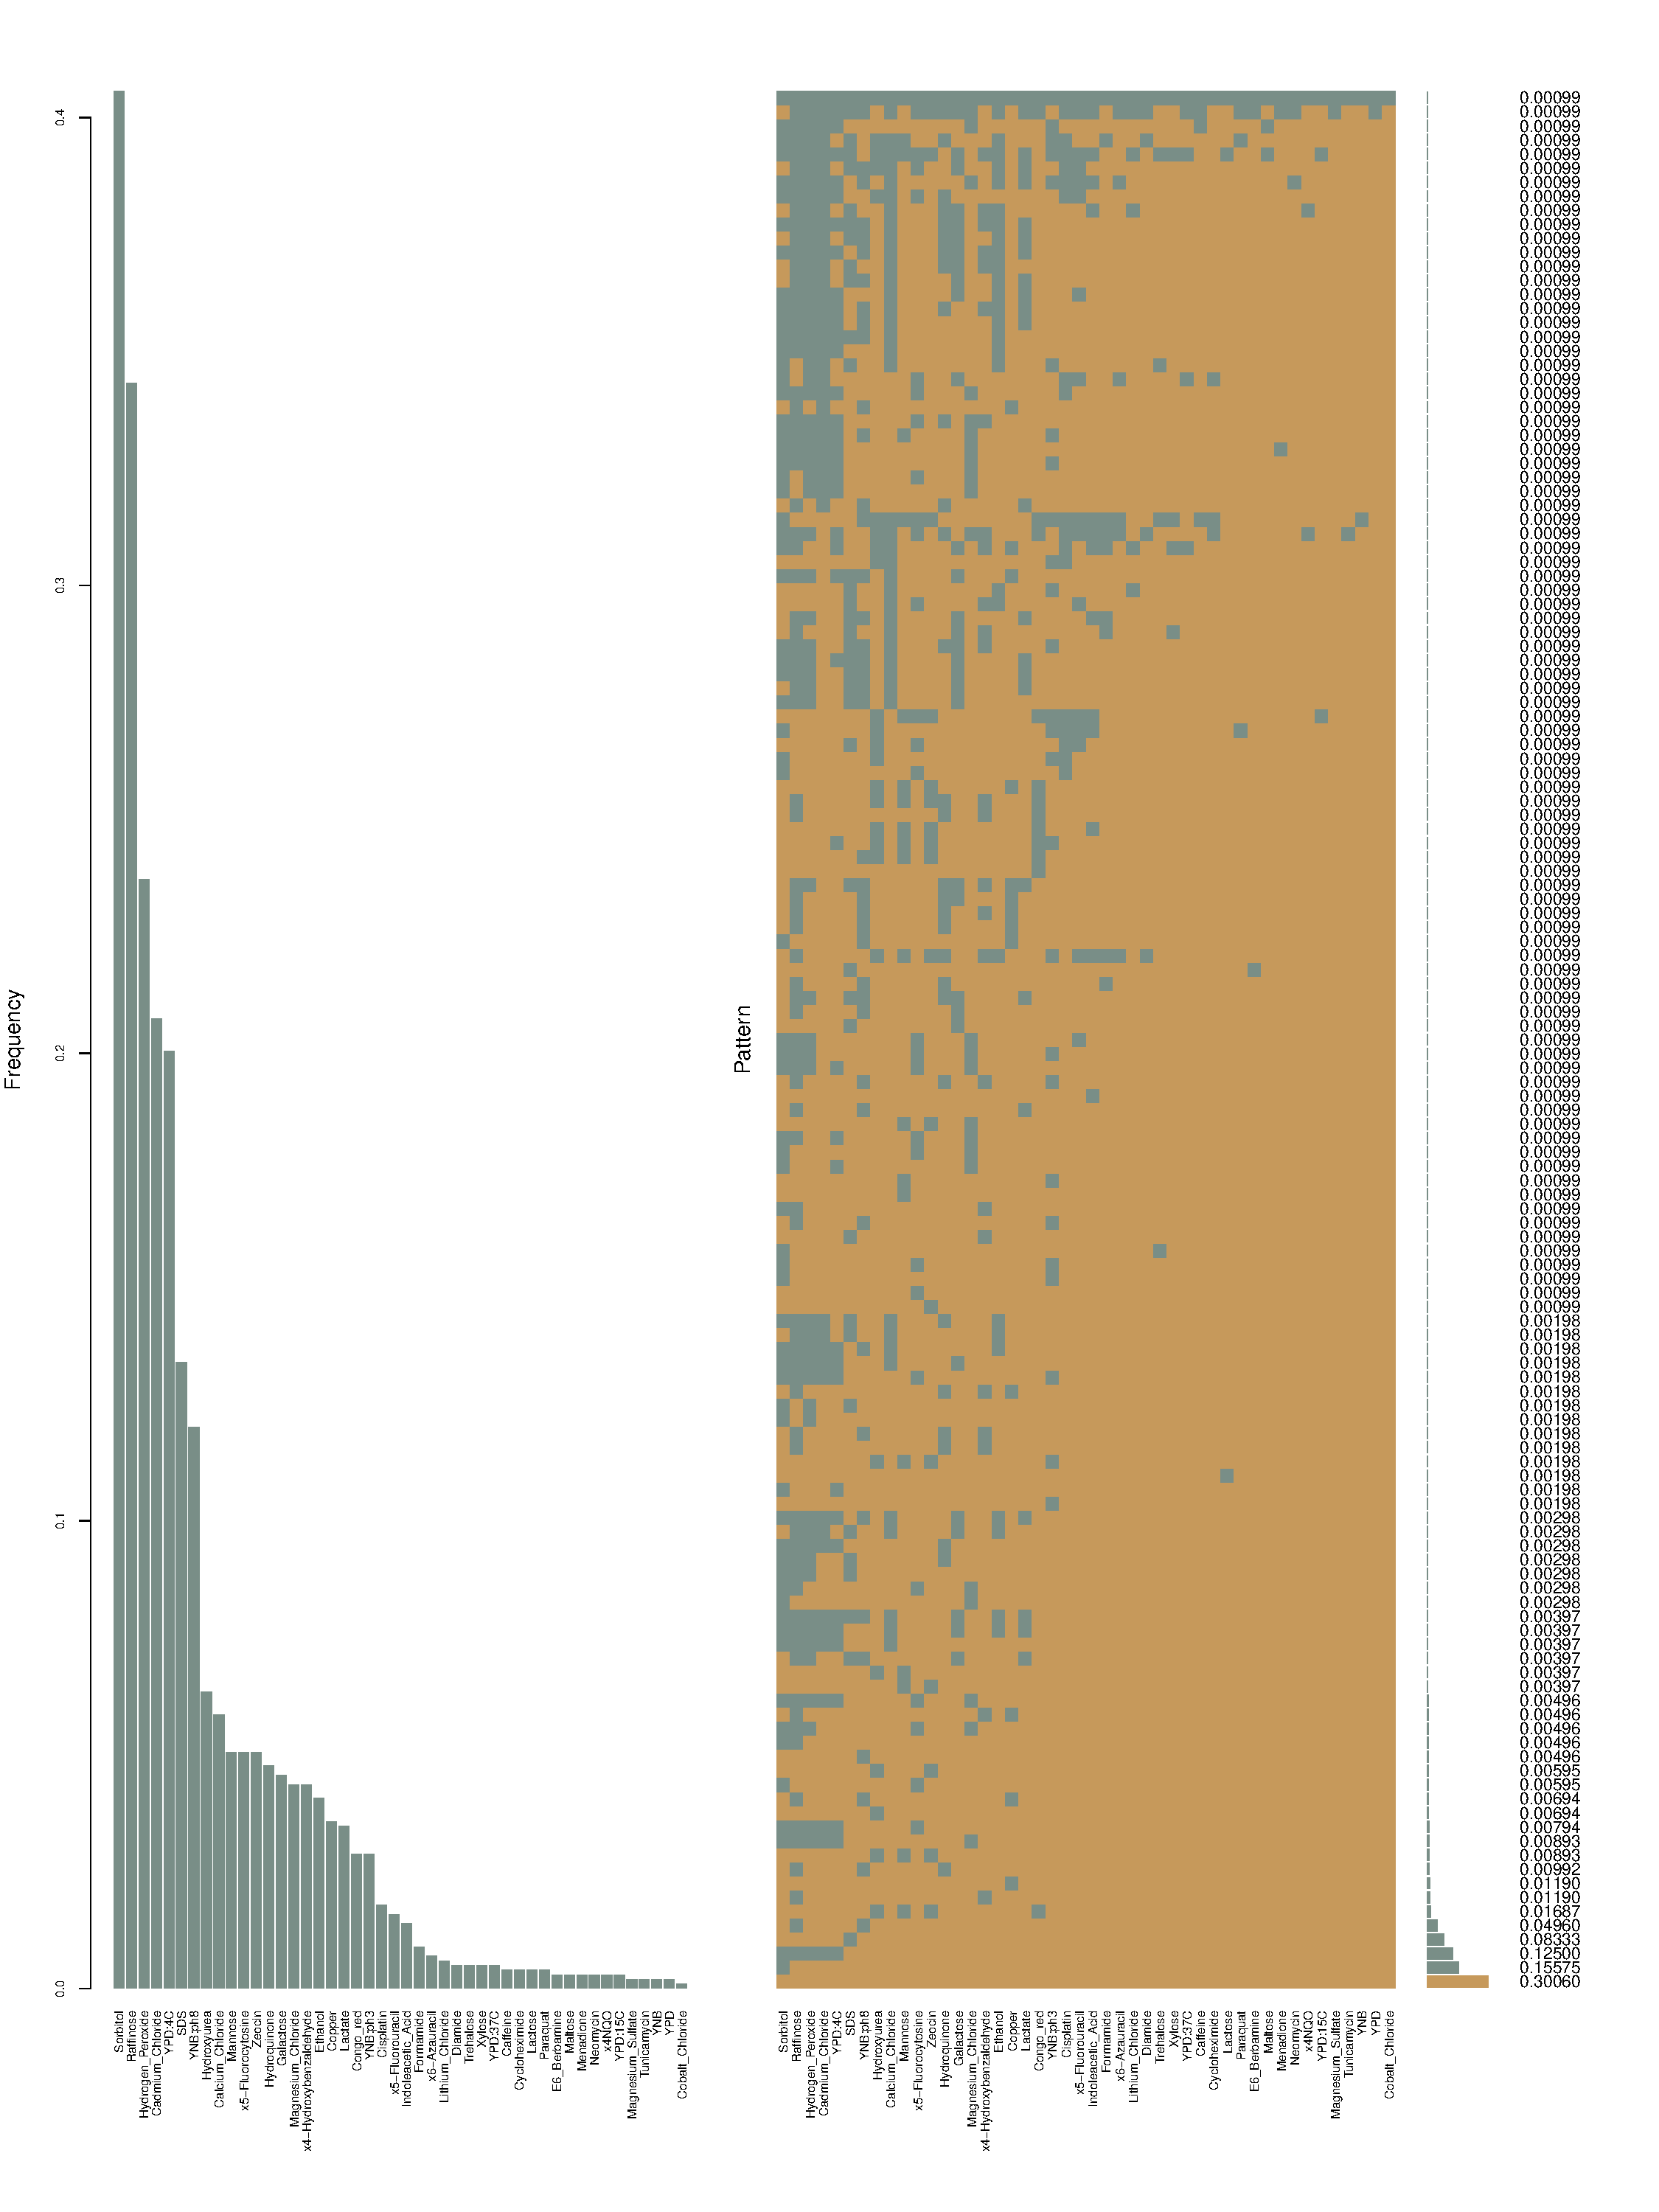
\includegraphics[trim = 0mm 0mm 20mm 2mm, clip, scale=0.2]{Chapter1/Figures/20170124_missing_data_pattern.pdf}
	\caption{\textbf{Full dataset}}
 		\label{fig:missingness-all}
	\end{subfigure}
	~
	\begin{subfigure}[b]{0.48\textwidth}
		%\hspace{3cm}
		\center
	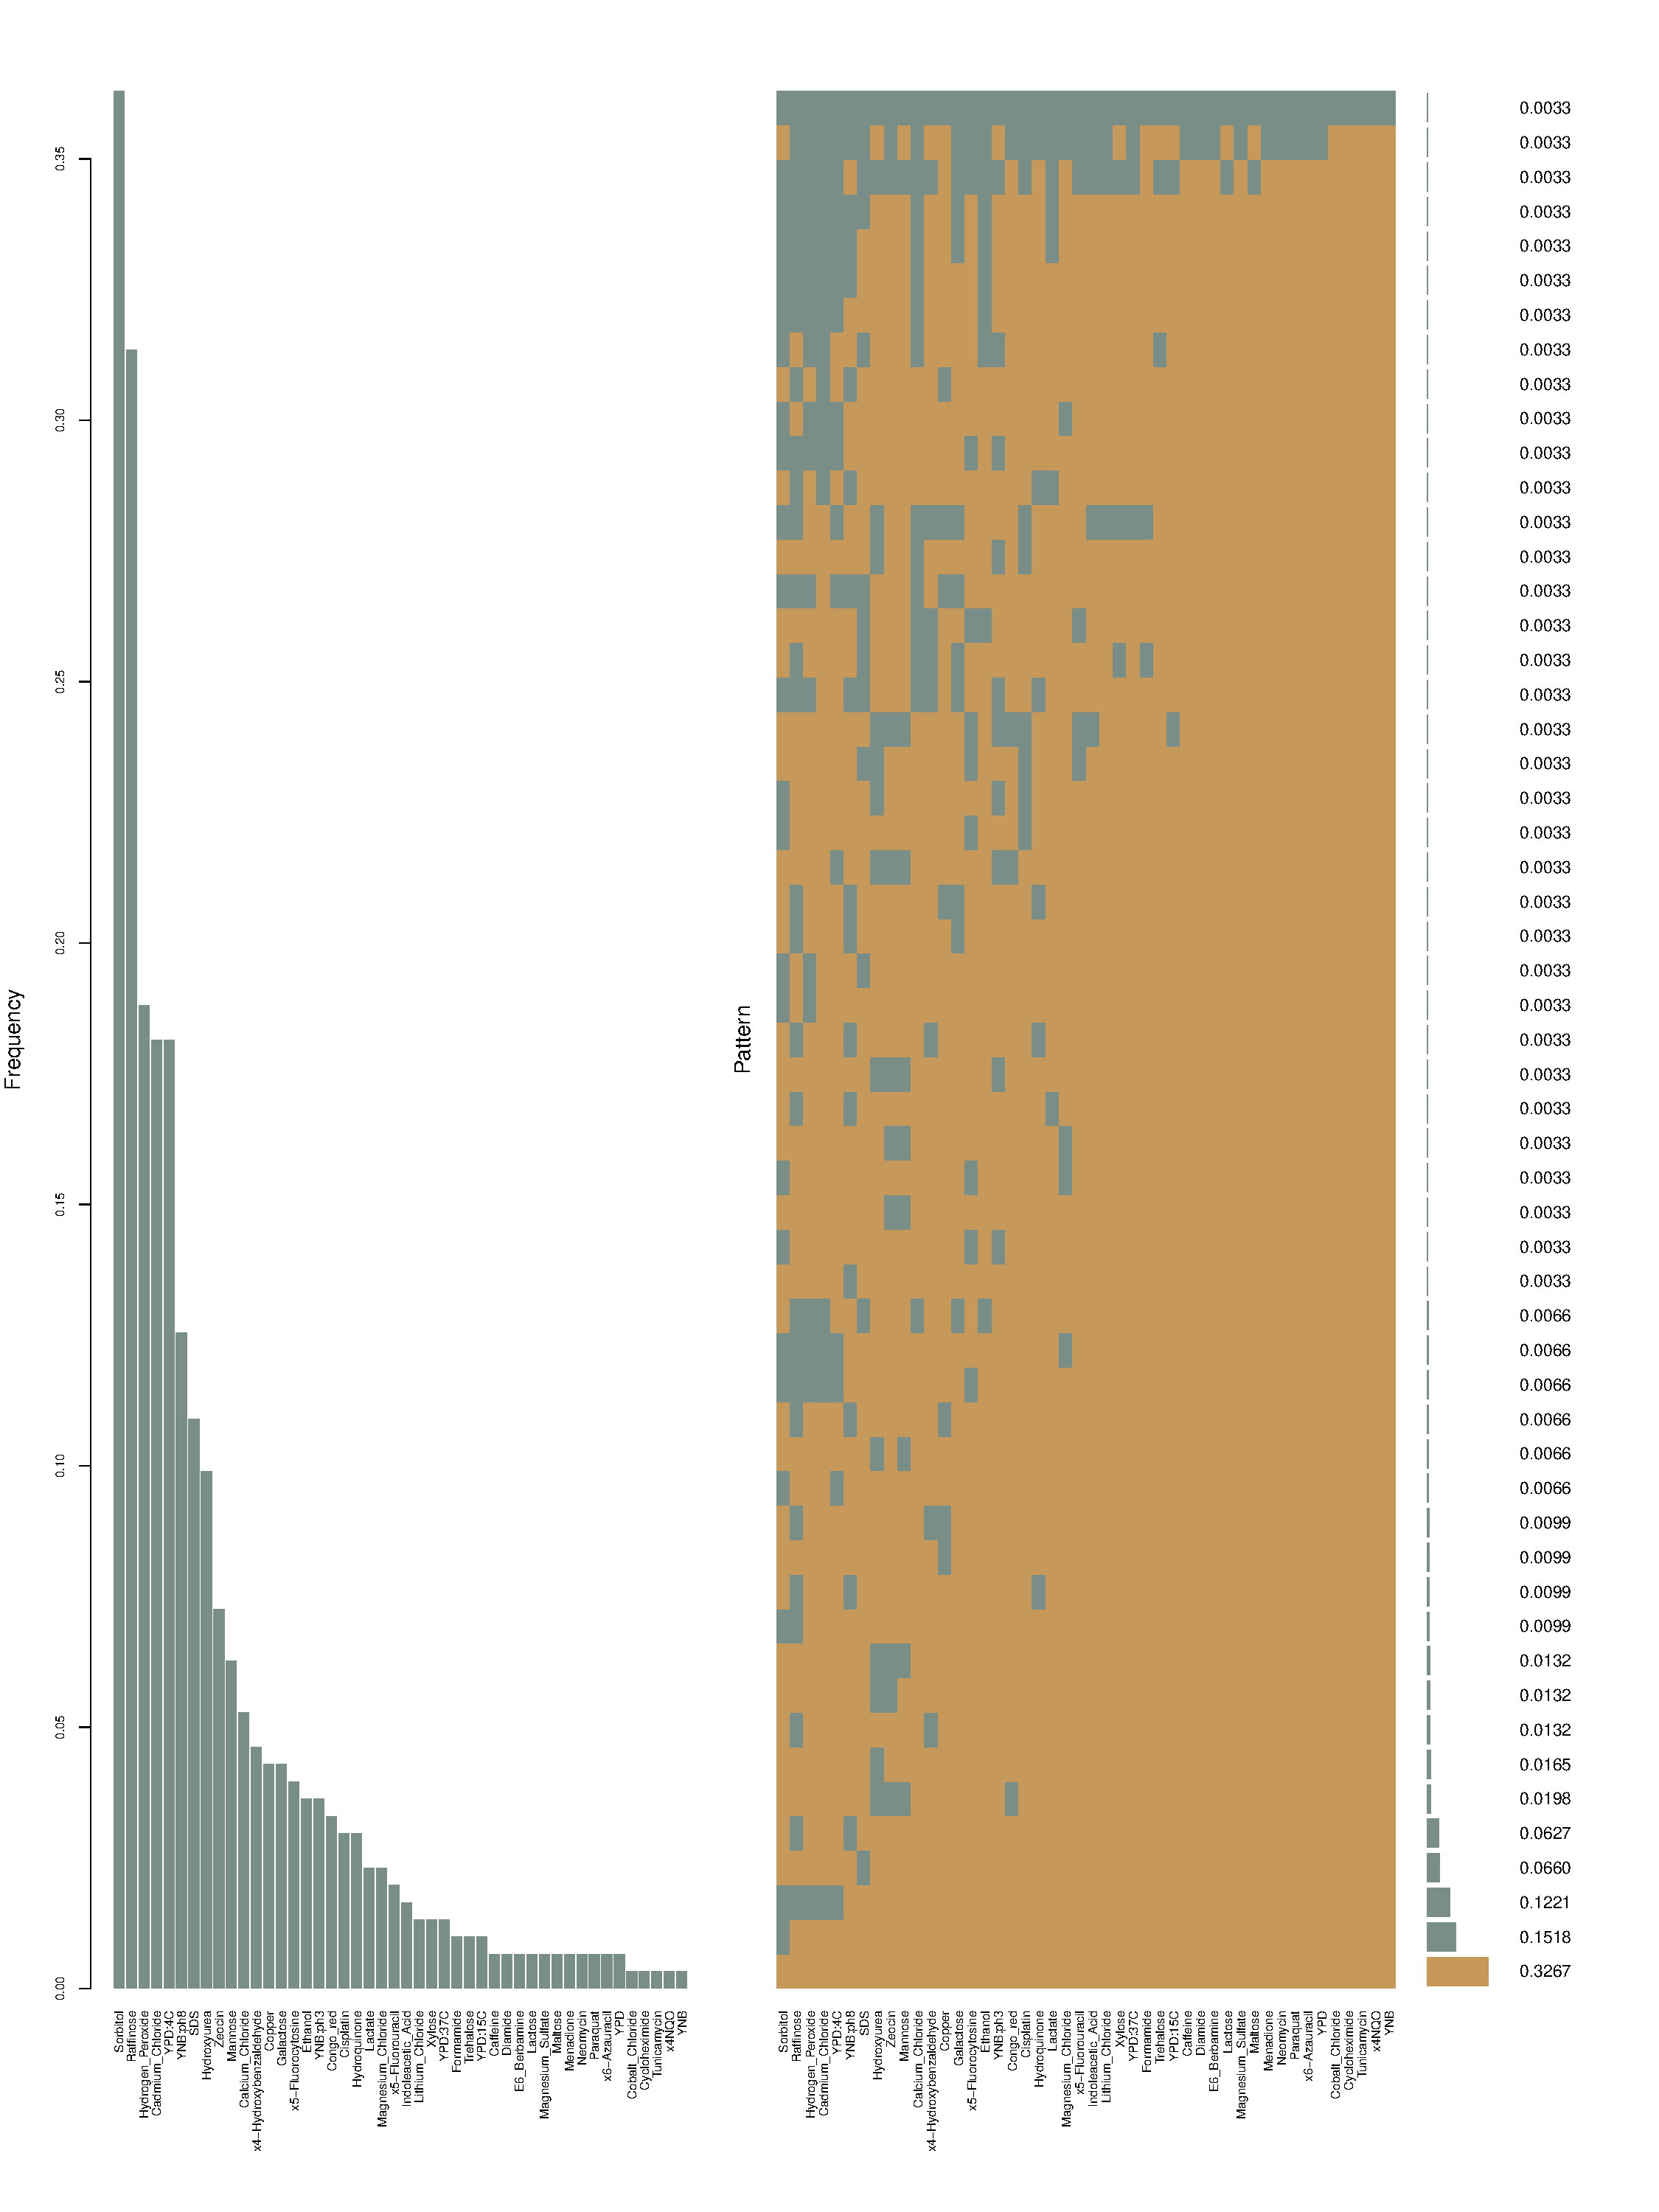
\includegraphics[trim = 0mm 0mm 20mm 2mm, clip, scale=0.2]{Chapter1/Figures/20170124_missing_data_pattern_simulated.pdf}\\
	\caption{\textbf{Simulated  dataset}}
 		\label{fig:missingness-sample}
	\end{subfigure}
	\caption[Frequencies and distributions of missing values in the yeast phenotype data]{\textbf{Frequencies and distributions of missing values in the yeast phenotype data.} In both panels, the histogram (left) shows the frequency of missing values for a particular trait. The aggregation plot (middle) depicts all existing combinations of missing and non-missing values in the traits. The bar chart and numbers (right) show the frequencies of occurrence of the different combinations (R Package: \emph{VIM} \citep{Templ2012}). (a) The full dataset contains normalised colony sizes for growth in 46 different conditions of 1,008 genotyped yeast segregants as derived from \citep{Bloom2013}. 306 segregants are fully genotyped (bar chart, orange bar). (b) Fully-phenotyped dataset of 306 segreagants with simulated missing values based on missingness patterns for then entire pool of 1,008 segregants.}
 	\label{fig:missingness}
\end{figure}

The LMM framework relies on all samples being fully genotyped and phenotyped and does not accept missing values. In order to use the largest possible subset of the data, I investigated imputation strategies for the missing phenotypes. I used the subset of 303 fully phenotyped samples to determine traits suitable for imputation. I simulated data with a similar pattern of missingness as observed in the original dataset by subsampling the full dataset to the subset size and overlaying the observed missingness pattern onto the subset of 303 fully phenotyped samples. The resulting pattern is depicted in Figure~\ref{fig:missingness-sample}. Similar results in frequencies of fully phenotyped samples and combination of missing/non-missing traits can be observed when comparing it to the original frequencies and patterns (Figure~\ref{fig:missingness-all}). I chose the MICE framework \citep{vanBuuren2011} with PMM as the imputation method to determine the most suitable imputation parameter settings in the simulated dataset which would then be applied to impute the real missing values in the full dataset. The predictor variables for each trait were determined based on its pair-wise Spearman's rank correlation coefficient \(\rho\) with all other traits in the dataset (Figure~\ref{fig:traitcorrelations}). In addition, only predictor traits that had been measured in at least 20\% of the samples in the dataset were considered. Different predictor variable set-ups were examined based on increasing thresholds for the Spearman's Rank correlation coefficient: \(\rho =\left\{0, 0.1, 0.2, 0.3\right\}\). Further parameters for MICE are the number of multiple iterations \(m\) (set to \(m=20\)) and the number of iterations \(maxit\) (set to \(maxit=30\)). For each predictor set-up, MICE was initiated with the same seed for the random number generator to ensure comparability. The goodness of the imputation was evaluated by computing the correlation of the imputed values (averaged across iterations \(m\)) to the experimentally observed ones. Traits where the imputed values correlated to the original ones by more then 95\% in at least one of the predictor set-ups were retained in the analysis. For five traits (cadmium chloride, hydrogen peroxide, raffinose, YNB:ph8, YPD:4C), no suitable predictors could be determined and these were excluded from further analyses (Figure~\ref{fig:mice}, red labels). For each trait, the predictor scheme that yielded the highest correlation between the imputed and observed data was chosen for the imputation of missing values in the full dataset. Missing values were imputed in segregants that were phenotyped for at least 80\% of the traits. The final dataset contained 981 segregants with phenotypes for 41 traits each. 

\begin{figure}[hbtp]
	\centering
	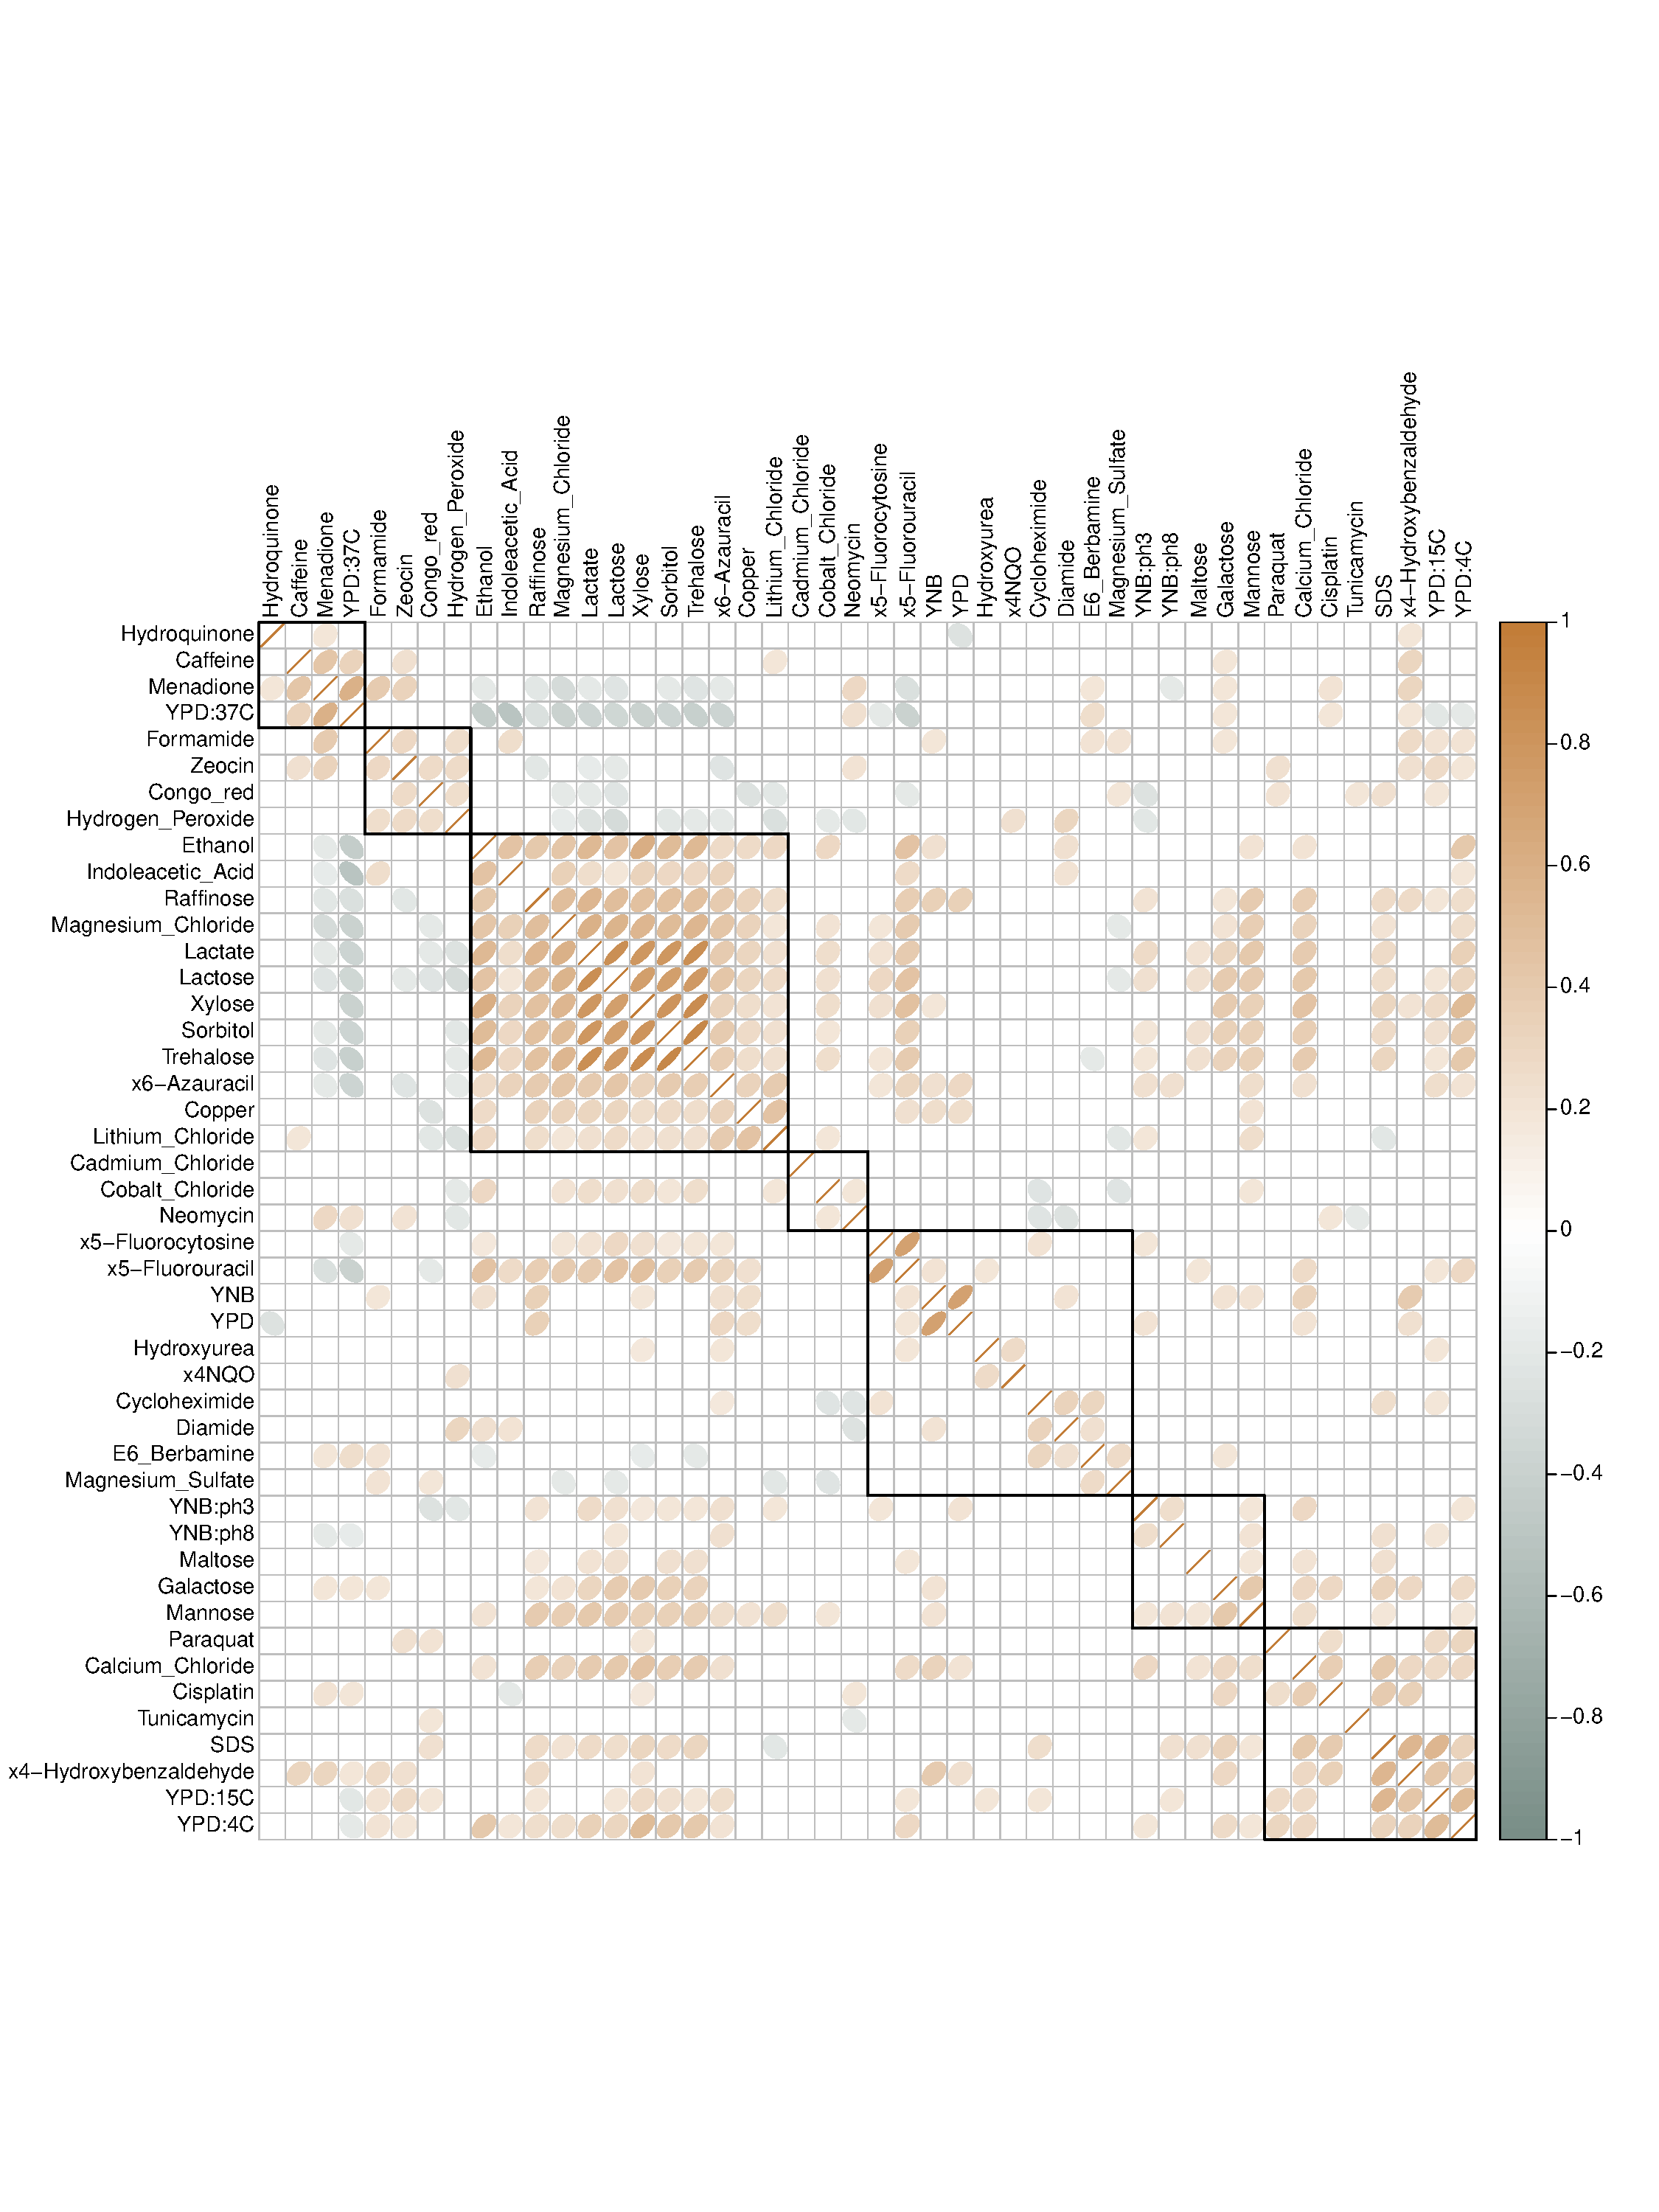
\includegraphics[trim = 0mm 80mm 10mm 80mm, clip, width=0.9\textwidth]{Chapter1/Figures/20170125_correlation_pheno_noNA.pdf}
	\caption[Pair-wise correlations of 46 growth traits in \emph{Saccharomyces cerevisiae}]{\textbf{Pair-wise correlations of 46 growth traits in \emph{Saccharomyces cerevisiae}.} For each trait pair, Spearman's rank correlation coefficient \(\rho\) and the p-values of the correlation were computed. The p-values were adjusted for multiple testing according to Benjamini and Hochberg's method \citep{Benjamini1995}. The strength and the direction of significant correlations (\(p < 0.05\)) are depicted above. Unsignificant correlations are left blank. The traits are clustered based on complete-linkage clustering of \((1-\rho)\) as distance measurement (R Package: \emph{corrplot}).}
 	\label{fig:traitcorrelations}
\end{figure}
 	
\begin{figure}[hbtp]
	\centering
	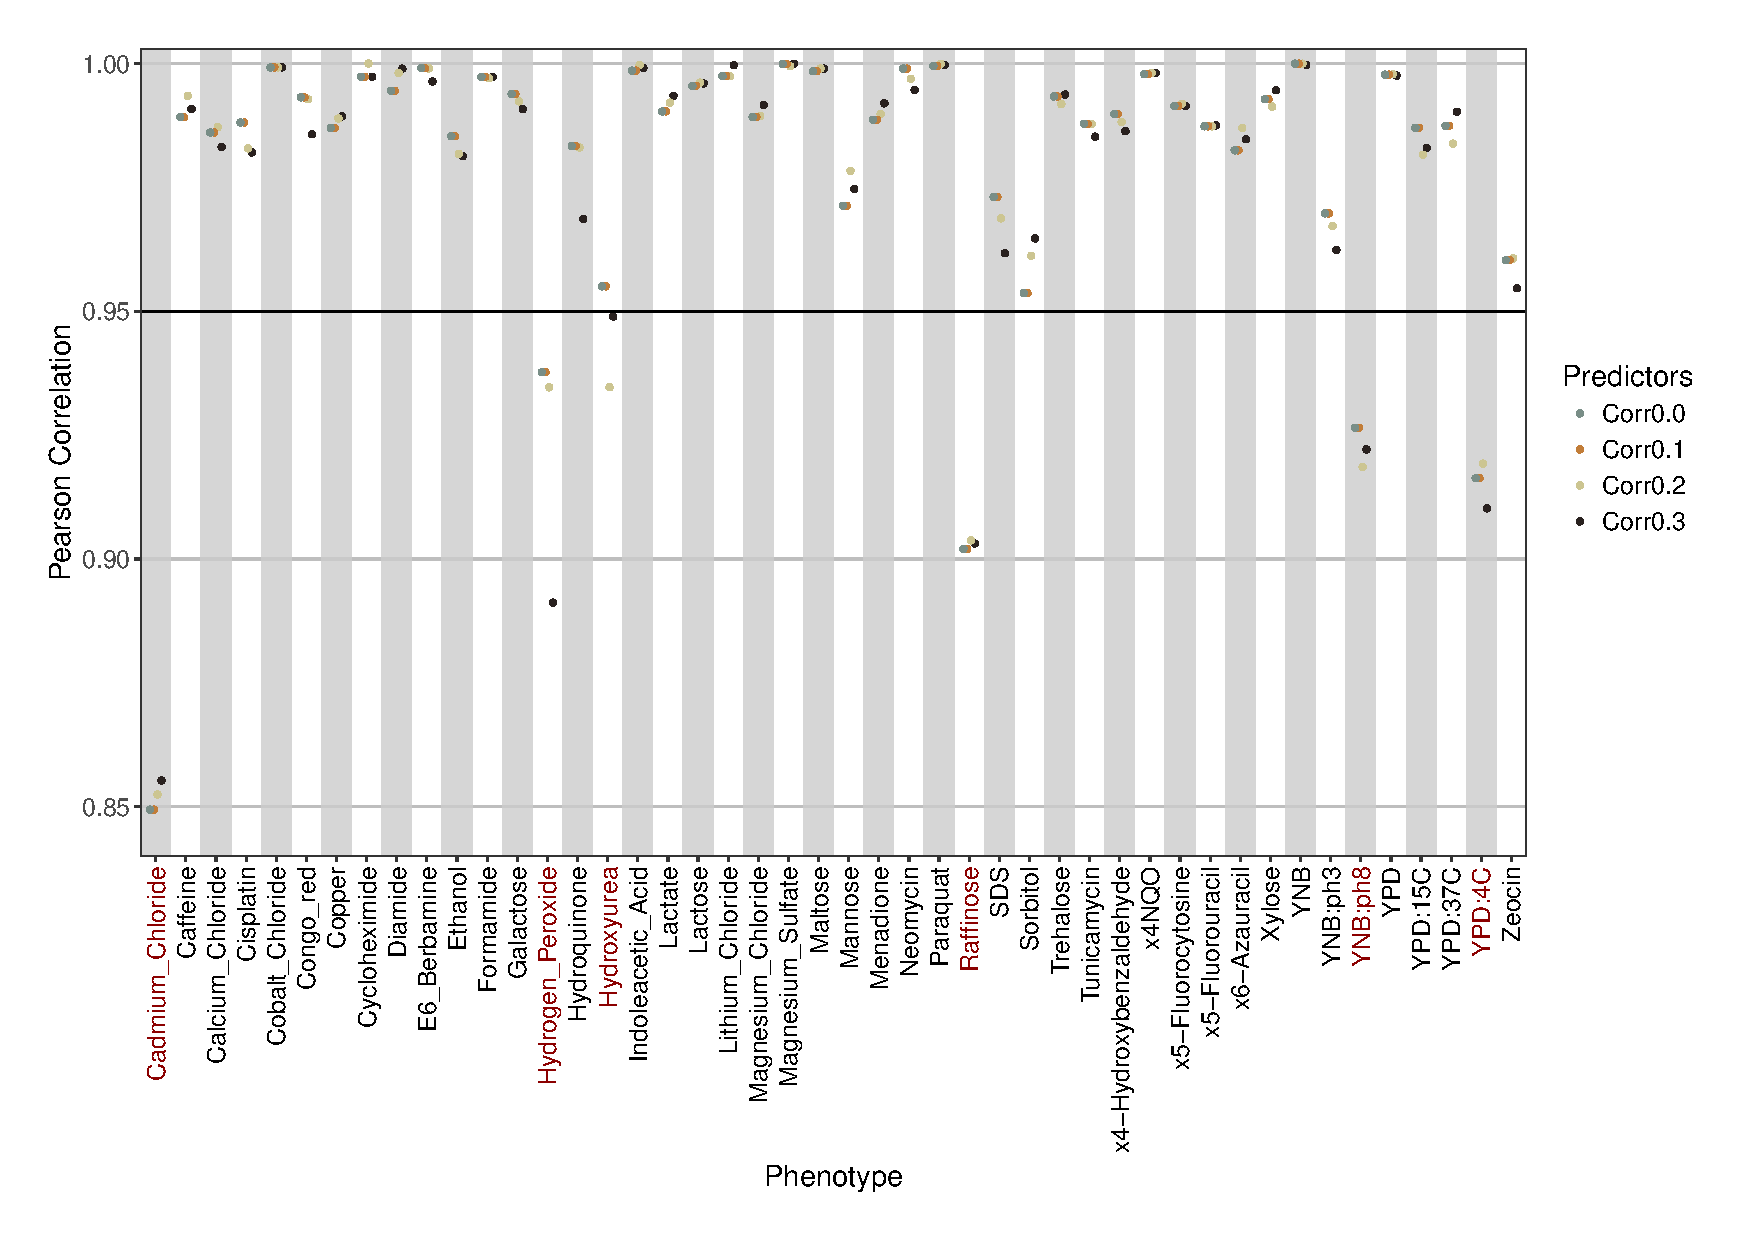
\includegraphics[trim = 0mm 0mm 0mm 0mm, clip, width=01\textwidth]{Chapter1/Figures/20170124_imputation_correlation_median_imputationvalue.pdf}
	\caption[Correlation between imputed and experimentally observed trait values]{\textbf{Correlation between imputed and experimentally observed trait values.} In the subset of 306 fully phenotyped samples, missing values were introduced and subsequently imputed via MICE. Different predictor sets were tested, differing in the predictors traits included. Sets were constructed based on different Spearman's rank correlation coefficient: traits were considered predictors if their correlation with the target trait was greater than a given threshold. For each predictor setup (\(\rho =\left\{0, 0.1, 0.2, 0.3\right\}\),   \(m=20\) multiple imputations and \(maxit=30\) iterations of MICE were conducted. The goodness of the imputation was evaluated by computing the correlation of the imputed values (averaged across iterations \(m\)) to the experimentally observed ones. Traits with at least one correlation greater than the 0.95 (black vertical line) were retained in the dataset. For traits labeled in red, the imputation was considered to be unreliable and the traits were excluded from further analyses (R Package: \emph{mice} \citep{vanBurren2011}).}
 	\label{fig:mice}
\end{figure}



\newpage
 \subsection{LiMMBo increases power in detecting genetic association in yeast}

\begin{itemize}
\item Assessing significance of association in yeast crosses via permutations \citep{Brehm2004, Ehrenreich2010}
\end{itemize} 
 
In order to test the performance of LiMMBo as a means for mtGWAS in a suitable set-up, i.e. in a cohort with related individuals, I conducted and compared an any effect mt-LMM-GWAS of 41 quantitative yeast traits to the results obtained in independent st-LMM-GWAS of the same traits. Figure~\ref{fig:GWAS-yeast} depicts the manhattan plot of both the st-LMM-GWAS p-values (adjusted for multiple testing by the effective number of tests \citep{Galwey2009}) and the mt-LMM-GWAS p-values. On several chromsomomes, mt-LMM-GWAS peaks (blue) are observed whereas no st-LMM-GWAS peaks (green) can be detected, demonstrating the increase in power by jointly modeling the traits. The heatmap below the mahattan plot shows the effect size estimates for each SNP for all 41 traits. Effect sizes were clustered based on their inner product across all SNPs. 
  \begin{figure}[hbtp]
	\centering
	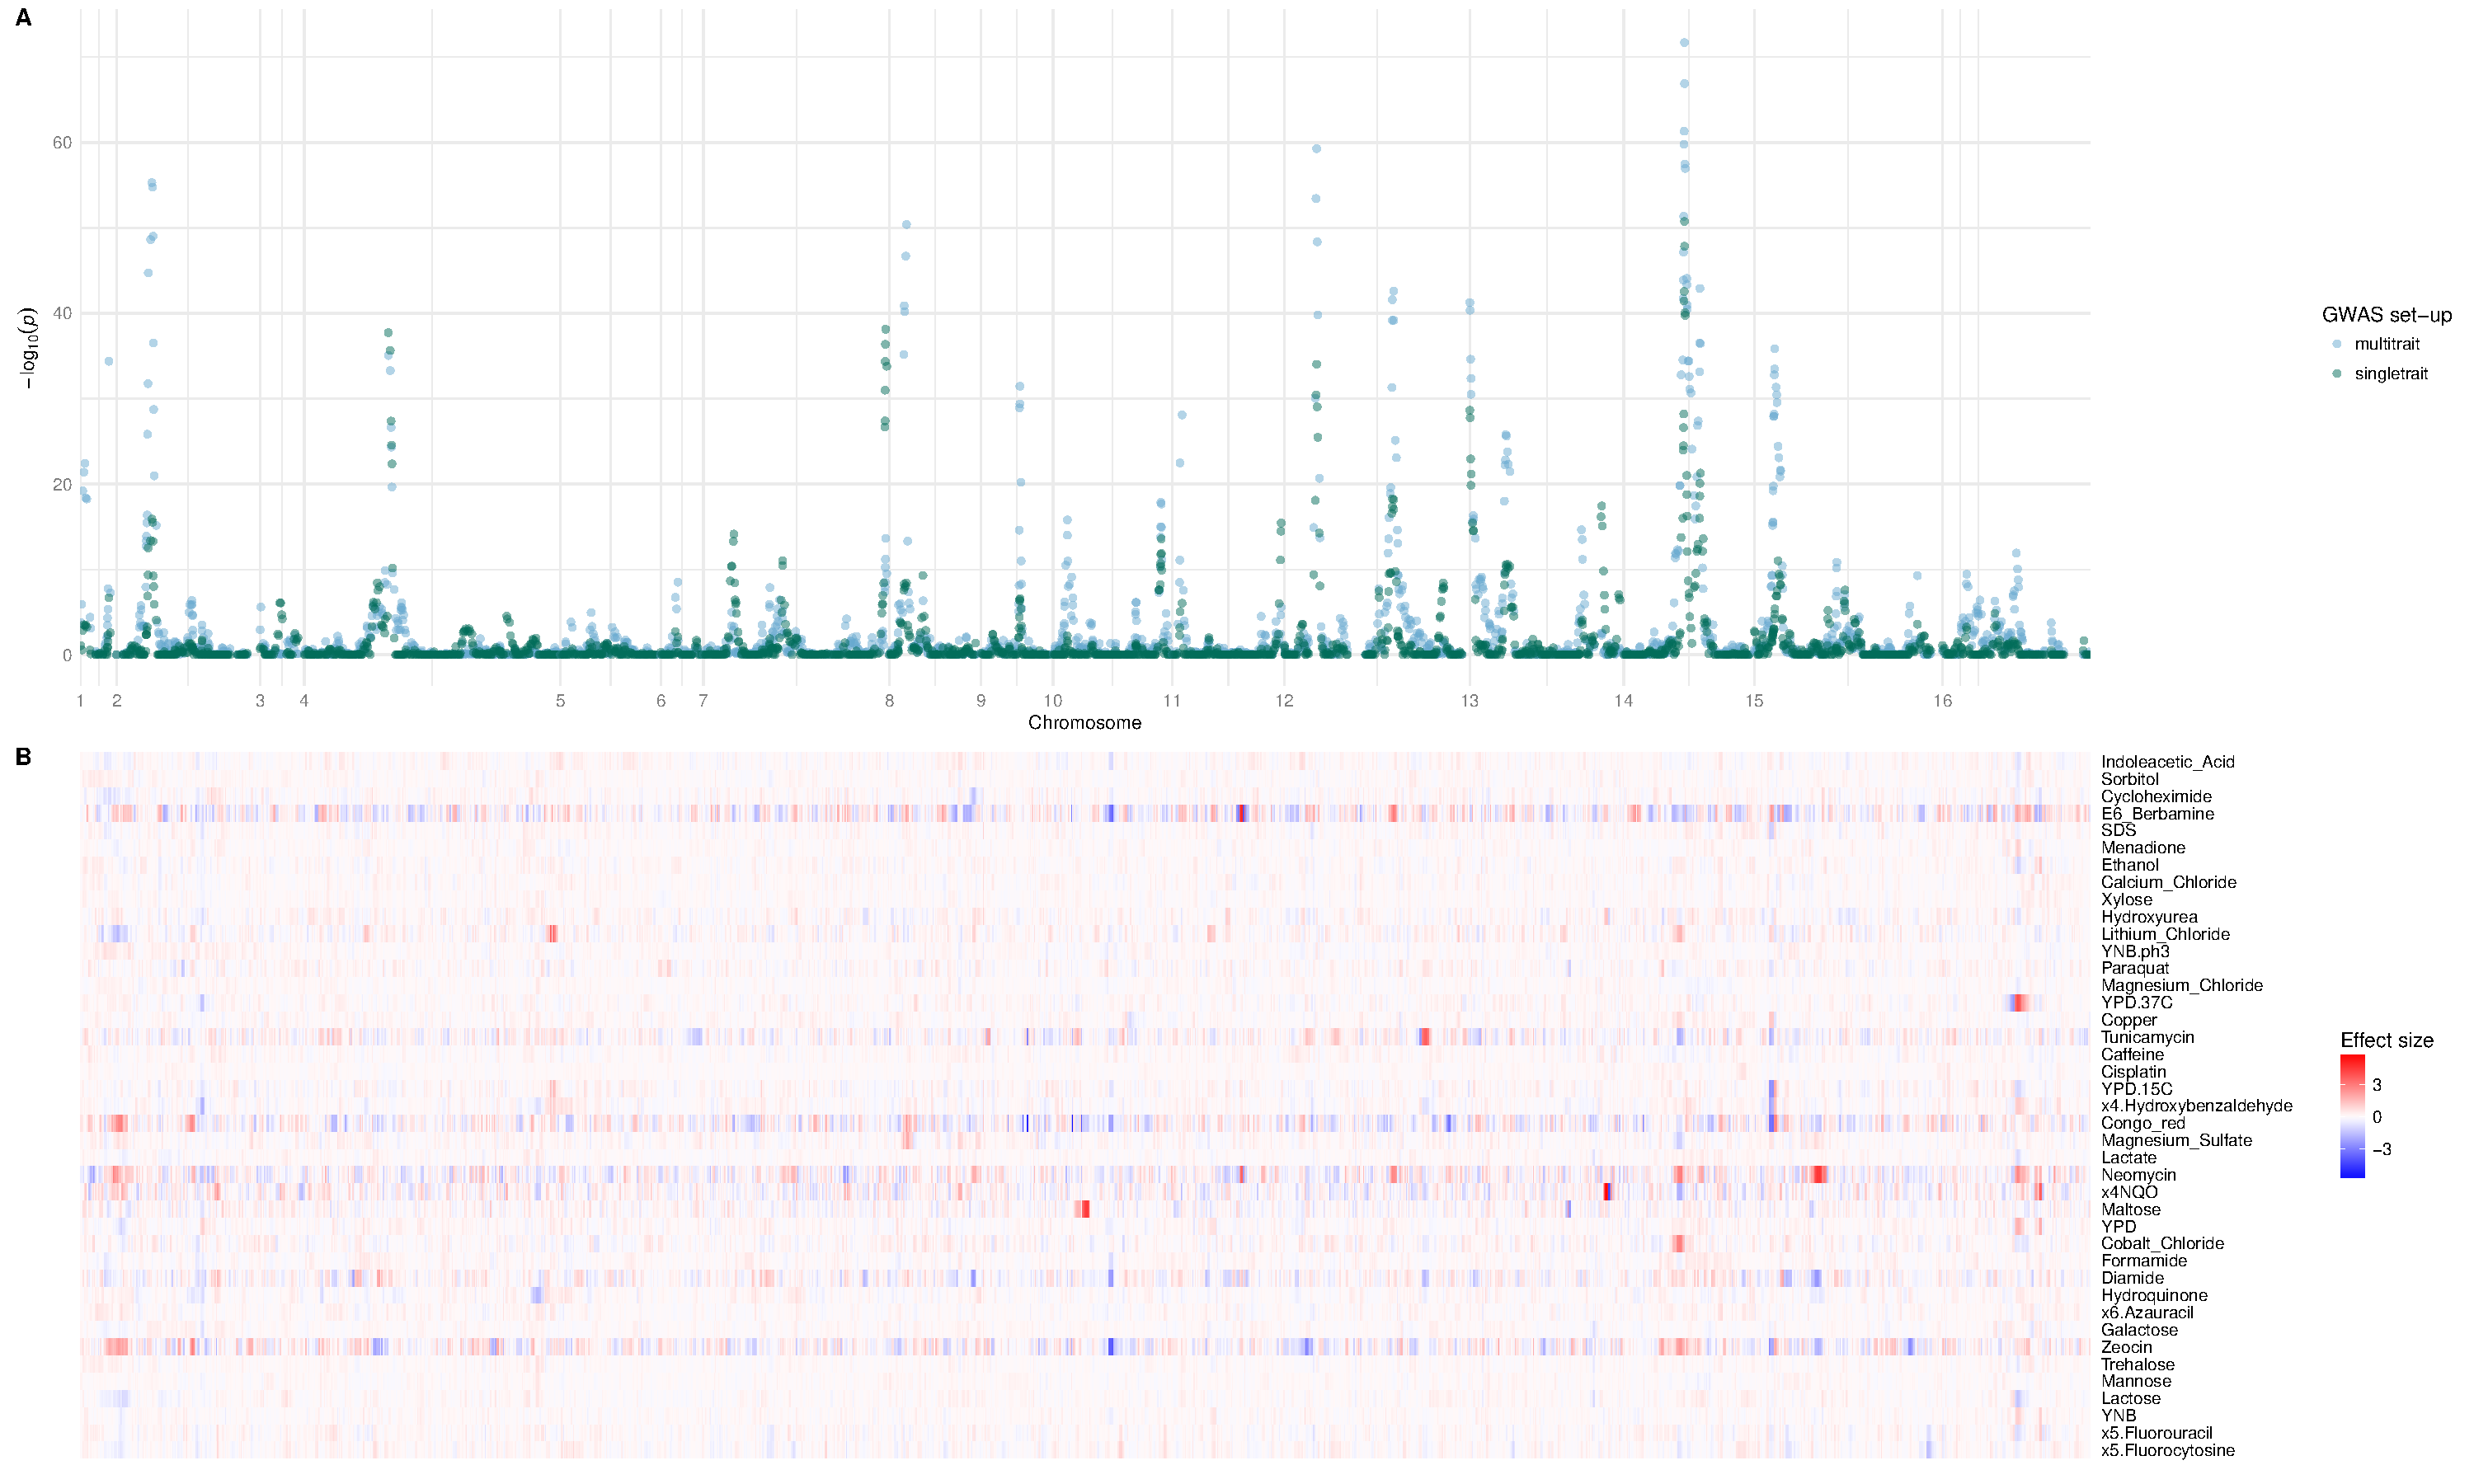
\includegraphics[trim = 0mm 0mm 0mm 0mm, clip, width=0.8\textwidth]{Chapter1/Figures/ManhattanEffectsizes.pdf}
	\caption[st-LMM-GWAS and any effect mt-LMM-GWAS of 41 quantitative traits in yeast]{\textbf{st-LMM-GWAS and any effect mt-LMM-GWAS of 41 quantitative traits in yeast.} (a) Manhattan plot of p-values from mt-LMM-GWAS (blue) and st-LMM-GWAS (green). Single-trait p-values are the minimum p-value per SNP for any of the 41 singletrait GWAS, adjusted for multiple testing by the effective number of test (\(T_{eff}=33\)). (b) Effect size estimates across the 41 jointly tested traits in the multitrait GWAS. Effect size estimate positions in the heatmap correspond the SNP positions in the manhattan plot.}
 	\label{fig:GWAS-yeast}
 	\end{figure}


%\subsection{Conclusion}
The simulation results show that Limmbo is effective in estimating large covariance matrices for multi-trait analysis. In a real, published dataset from yeast, I can show an increase in power by detecting new loci that could not be associated in single-trait analysis. As well as the gain in power, the analysis provides a more integrated view of the relationships between loci, with a number of loci showing similar beta-patterns, suggesting that they are part of the same biological mechanism. Interestingly, all linear mixed models probably require some level of population structure to form good estimates of the trait-by-trait covariance structure of the background effects; in situations with low levels of population structure the simpler approach of a linear model without a covariance matrix is better calibrated. Overall I have shown that Limmbo is a robust method for large scale trait analysis with benefits in real world settings.


\bibliography{myLibrary2}
\bibliographystyle{ebi}

\beginsupplement
\section{Quality control: genotyping}

\begin{figure}[hbtp]
	\centering
	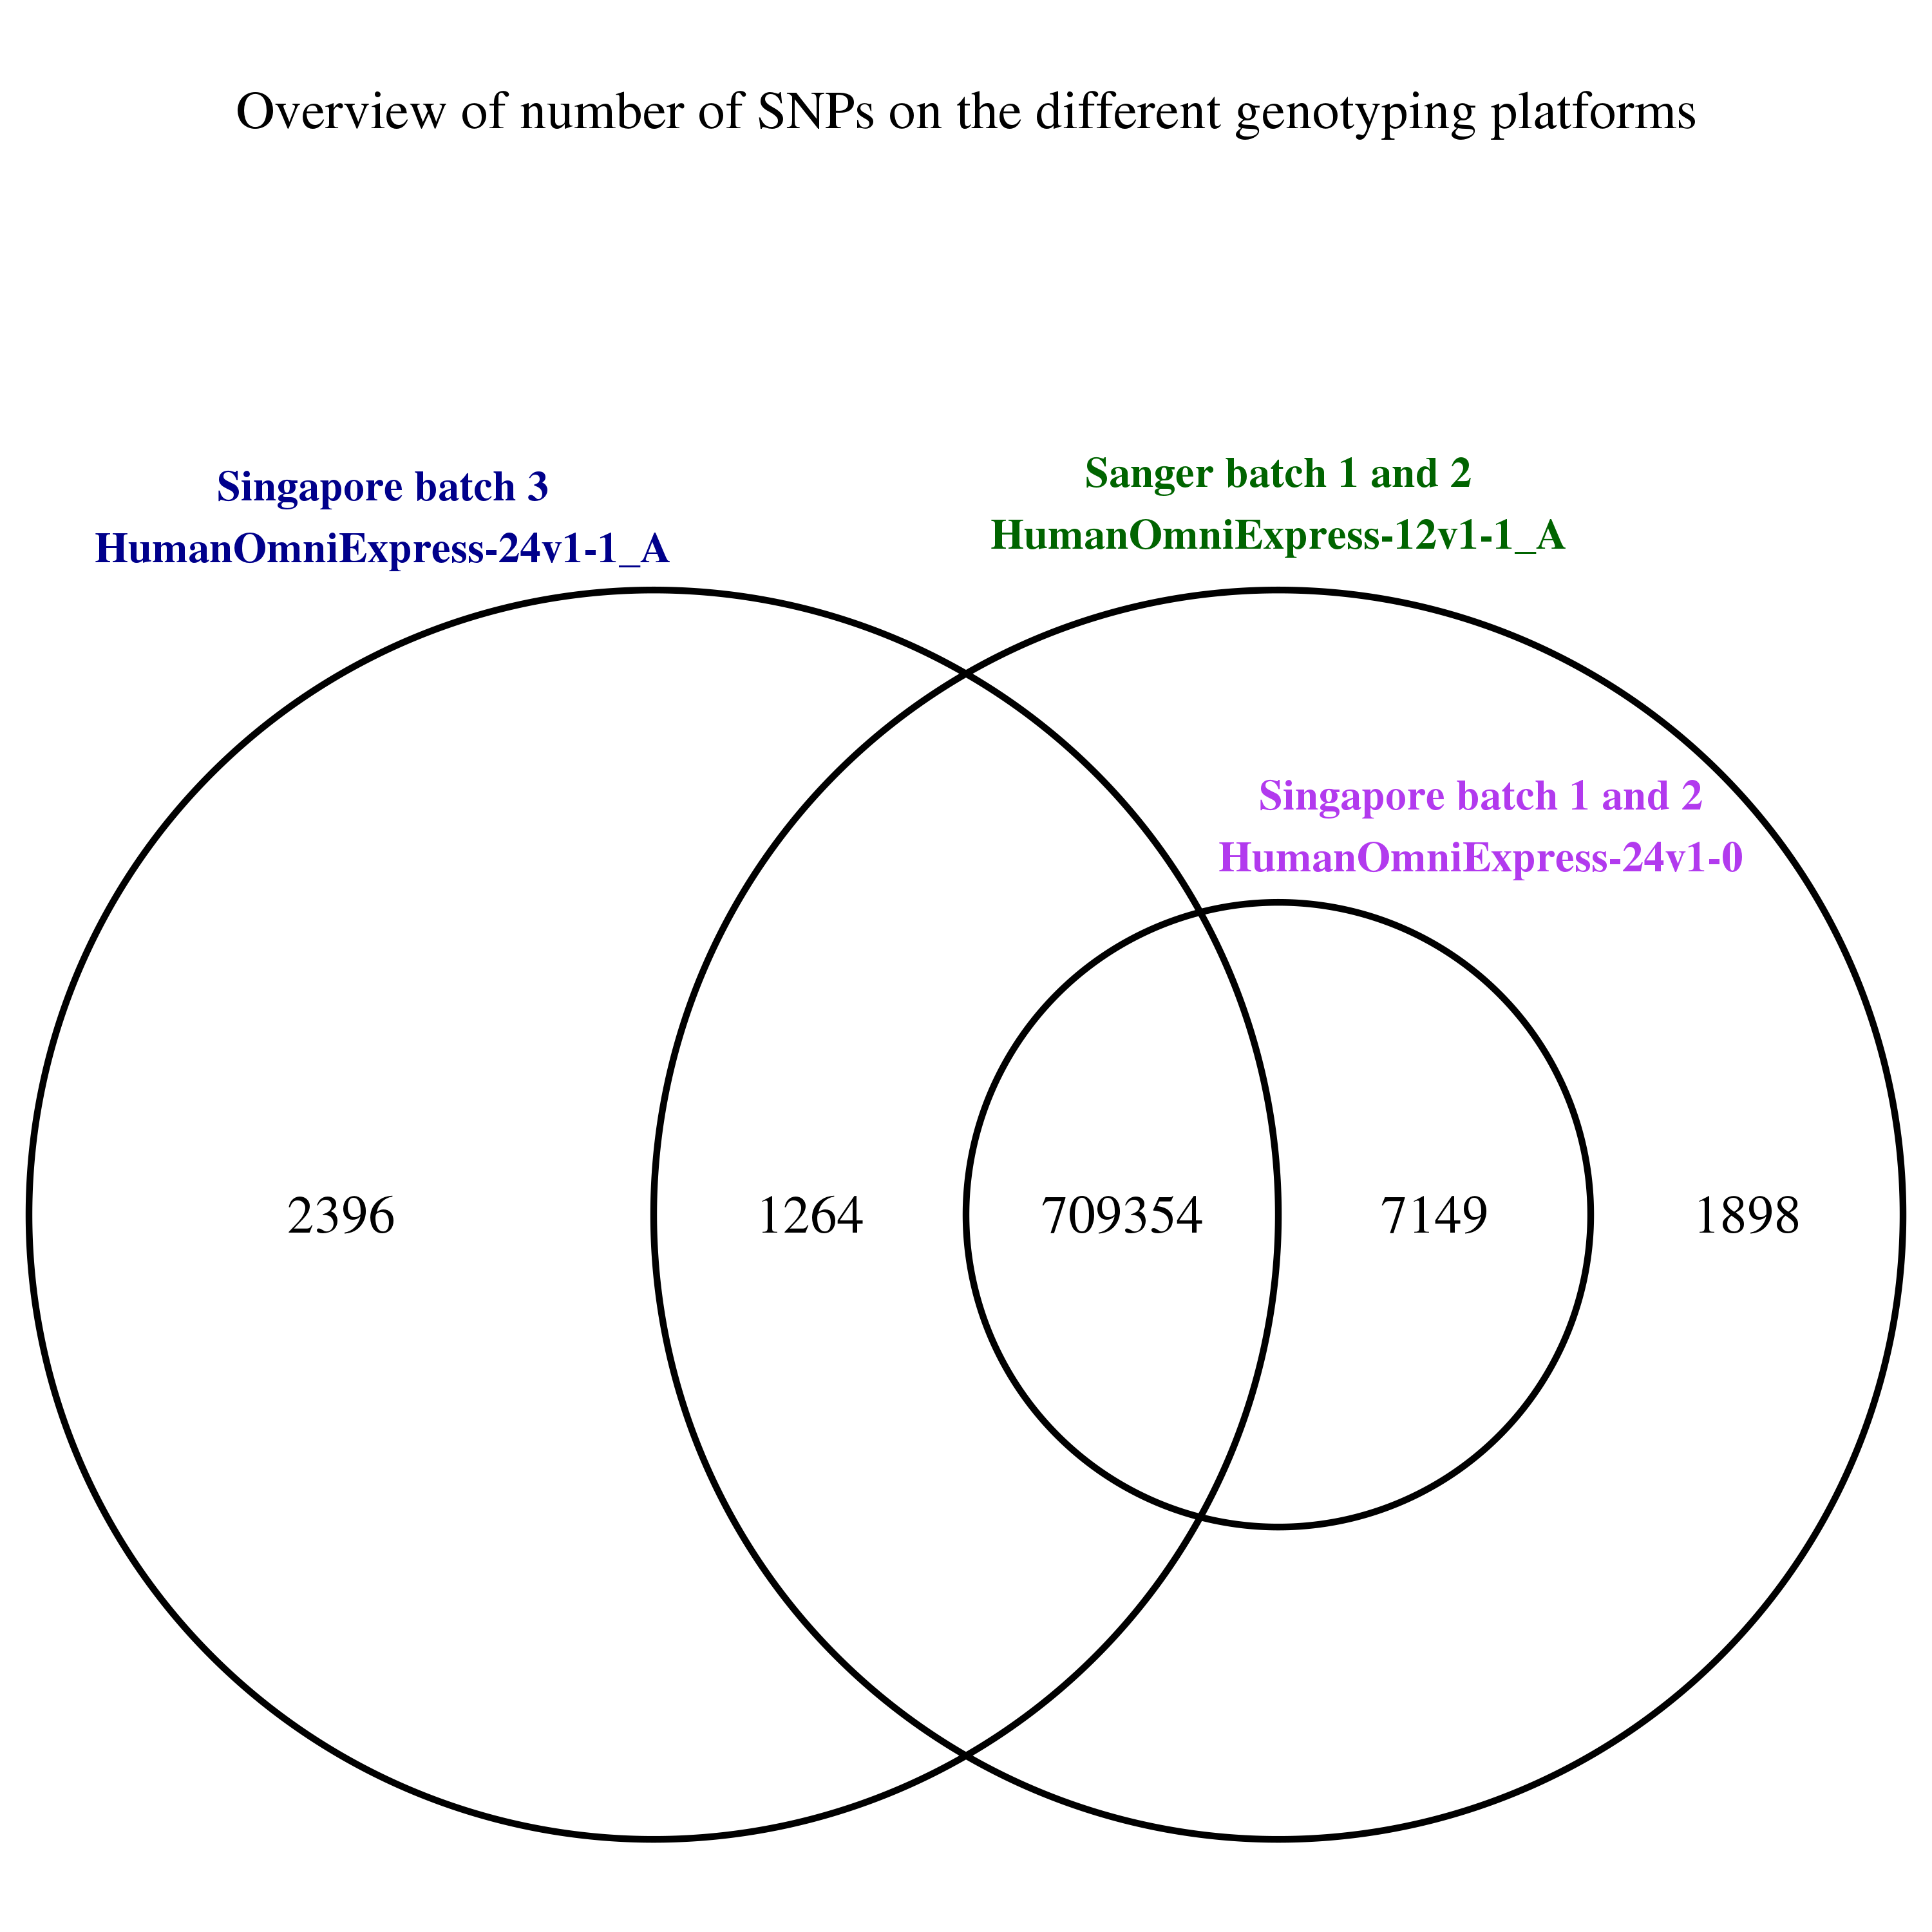
\includegraphics[trim = 0mm 0mm 0mm 20mm, clip, width=0.8\textwidth]{Figures/Venn_genotyping_batches.png}
	\caption{\textbf{.} .}
 	\label{fig:probeoverlap}
\end{figure}

\begin{figure}[hbtp]
	\centering
	\includegraphics[trim = 0mm 0mm 0mm 20mm, clip, width=0.8\textwidth]{Figures/SampleQC.pdf}
	\caption{\textbf{.} .}
 	\label{fig:sampleQC}
\end{figure}

\begin{figure}[hbtp]
	\centering
	\includegraphics[trim = 0mm 0mm 0mm 20mm, clip, width=0.8\textwidth]{Figures/SNPQC.pdf}
	\caption{\textbf{.} .}
 	\label{fig:SNPQC}
\end{figure}

\begin{figure}[hbtp]
	\centering
	\includegraphics[trim = 0mm 0mm 0mm 20mm, clip, width=0.8\textwidth]{Figures/kinshipQC.pdf}
	\caption{\textbf{.} .}
 	\label{fig:kinshipQC}
\end{figure}

\section{Quality control: imputation}

\begin{figure}[hbtp]
	\centering
	\includegraphics[trim = 0mm 0mm 0mm 20mm, clip, width=0.8\textwidth]{Figures/perBatchSNPsperChr.pdf}
	\caption{\textbf{.} .}
 	\label{fig:imputeQC}
\end{figure}
\end{document}


